% Sablon pentru realizarea lucrarii de licenta, conform cu recomandarile
% din ghidul de redactare:
% - https://fmi.unibuc.ro/finalizare-studii/
% - https://drive.google.com/file/d/1xj9kZZgTkcKMJkMLRuoYRgLQ1O8CX0mv/view

% Multumiri lui Gabriel Majeri, acest sablon a fost creat pe baza
% codului sursa a lucrarii sale de licenta. 
% Codul sursa: https://github.com/GabrielMajeri/bachelors-thesis
% Website: https://www.gabrielmajeri.ro/
%
% Aceast sablon este licentiat sub Creative Commons Attribution 4.0 International License.

\documentclass[12pt, a4paper]{report}

% Suport pentru diacritice și alte simboluri
\usepackage{fontspec}
\usepackage{ dsfont }

% Suport pentru aranjarea imaginilor
\usepackage{float}

% Suport pentru anexe
\usepackage{appendix}

% Suport pentru mai multe limbi
\usepackage{polyglossia}

% Setează limba textului la română
\setdefaultlanguage{romanian}
% Am nevoie de engleză pentru rezumat
\setotherlanguages{english}

% Indentează și primul paragraf al fiecărei noi secțiuni
\SetLanguageKeys{romanian}{indentfirst=true}

% Suport pentru diferite stiluri de ghilimele
\usepackage{csquotes}

\DeclareQuoteStyle{romanian}
  {\quotedblbase}
  {\textquotedblright}
  {\guillemotleft}
  {\guillemotright}

% Utilizează biblatex pentru referințe bibliografice
\usepackage[
    maxbibnames=50,
    sorting=nty
]{biblatex}

\addbibresource{bibliography.bib}

% Setează spațiere inter-linie la 1.5
\usepackage{setspace}
\onehalfspacing

% Modificarea geometriei paginii
\usepackage{geometry}

% Include funcțiile de grafică
\usepackage{graphicx}
% Încarcă imaginile din directorul `images`
\graphicspath{{./images/}}

% Listări de cod
\usepackage{listings}

% Linkuri interactive în PDF
\usepackage[
    colorlinks,
    linkcolor={black},
    menucolor={black},
    citecolor={black},
    urlcolor={blue}
]{hyperref}

% Simboluri matematice codificate Unicode
\usepackage[warnings-off={mathtools-colon,mathtools-overbracket}]{unicode-math}

% Comenzi matematice
\usepackage{amsmath}
\usepackage{mathtools}

% Formule matematice
\newcommand{\bigO}[1]{\symcal{O}\left(#1\right)}
\DeclarePairedDelimiter\abs{\lvert}{\rvert}

% Suport pentru rezumat în două limbi
% Bazat pe https://tex.stackexchange.com/a/70818
\newenvironment{abstractpage}
  {\cleardoublepage\vspace*{\fill}\thispagestyle{empty}}
  {\vfill\cleardoublepage}
\renewenvironment{abstract}[1]
  {\bigskip\selectlanguage{#1}%
   \begin{center}\bfseries\abstractname\end{center}}
  {\par\bigskip}

% Stiluri diferite de headere și footere
\usepackage{fancyhdr}

% Metadate
\title{Agent pentru Monopoly bazat pe reinforcement learning}
\author{Ocnaru Mihai-Octavian}

% Generează variabilele cu @
\makeatletter

\begin{document}

% Front matter
\cleardoublepage
\let\ps@plain

% Pagina de titlu
\begin{titlepage}

% Redu marginile
\newgeometry{left=2cm,right=2cm,bottom=1cm}

\begin{figure}[!htb]
    \centering
    \begin{minipage}{0.2\textwidth}
        
\includegraphics[width=\linewidth]{logo-ub.png}
    \end{minipage}
    \begin{minipage}{0.5\textwidth}
        \large
        \vspace{0.2cm}
        \begin{center}
            \textbf{UNIVERSITATEA DIN BUCUREȘTI}
        \end{center}
        \vspace{0.3cm}
        \begin{center}
            \textbf{
                FACULTATEA DE \\
                MATEMATICĂ ȘI INFORMATICĂ
            }
        \end{center}
    \end{minipage}
    \begin{minipage}{0.2\textwidth}
        
\includegraphics[width=\linewidth]{logo-fmi.png}
    \end{minipage}
\end{figure}

\begin{center}
\textbf{SPECIALIZAREA INFORMATICĂ}
\end{center}

\vspace{1cm}

\begin{center}
\Large \textbf{Lucrare de licență}
\end{center}

\begin{center}
\huge \textbf{\MakeUppercase{\@title}}
\end{center}

\vspace{3cm}

\begin{center}
\large \textbf{Absolvent \\ \@author}
\end{center}

\vspace{0.25cm}

\begin{center}
\large \textbf{Coordonator științific \\ Conf.dr. Mihai Prunescu}
\end{center}

\vspace{2cm}

\begin{center}
\Large \textbf{București, iunie 2025}
\end{center}
\end{titlepage}
\restoregeometry
\newgeometry{
    margin=2.5cm
}

\fancypagestyle{main}{
  \fancyhf{}
  \renewcommand\headrulewidth{0pt}
  \fancyhead[C]{}
  \fancyfoot[C]{\thepage}
}

\addtocounter{page}{1}

% Rezumatul
\begin{abstractpage}
\vspace*{\fill}
\begin{abstract}{romanian}

Datorită avansării și progresului tehnologic, procesarea și resursele computaționale au facilitat avântul în direcția dezvoltării capacităților inteligenței artificiale. Astfel o arie ce a început să se remarce în ultimii ani prin explorarea și dezvoltarea noilor posibilități este învățarea prin întărire (reinforcement learning). Aceasta presupune antrenarea unui agent inteligent ce are ca scop navigarea printr-un spațiu (environment) și interacțiunea cu acesta într-o formă ce maximizează un scop predefinit.

Jocul Monopoly este un candidat perfect pentru ilustrarea și modelarea unui agent care să descopere o strategie proprie și să creeze o politică de interacționare inteligentă. Datorită gradului de complexitate ridicată, favorizată de spațiul mare de acțiuni și stări posibile, al impredictibilității datorate aruncării zarurilor și extragerii cartonașelor „Cufărul comunității" și „Șansa", dar și al strategiilor de abordare a jocului nelimitate, construirea unui model al jocului care să funcționeze optim este o provocare care nu poate fi depășită ușor decât printr-o abordare dinamică.

Dat fiind gradul ridicat de complexitate și componenta aleatorie, pentru facilitarea învățării și deprinderea unei bune cunoașteri a mediului, dar și generarea unei politici optime, vom folosi o abordare hibridă ce presupune derivarea agentului inteligent dintr-un agent cu o strategie algoritmică și fixă. Implementarea hibridă va asigura că vom putea folosi metodele părintelui în cazul acțiunilor cu un spațiu mare de posibilități ce ar fi îngreunat atât modelarea mediului cât și învățarea unei strategii bune, iar pe cele deprinse prin explorarea environment-ului le vom folosi pentru cele ce au putut fi modelate cu ușurință.

Implementarea agentului de reinforcement learning se va face folosind o rețea adâncă de tipul Q (Deep Q-network, DQN), utilizând o paradigmă hibridă de învățare. Prima dată rețeaua va fi antrenată într-o manieră supervizată, folosind mai mulți agenți experți (expert learning), iar mai apoi aceasta își va continua antrenamentul interacționând cu mediul direct. O nouă îmbunătățire adusă arhitecturii este folosirea mai multor rețele pentru fiecare acțiune întreprinsă, lucru ce favorizează focalizarea, ajutând la particularizarea politicii optime.

Rezultatele obținute arată că prin această arhitectură și abordare agentul inteligent reușește să depășească agentul părinte cu politica statică, atingând o rată de victorie de 90\% împotriva sa și depășindu-l pe acesta cu 5,3 procente într-un turneu cu 12 agenți, într-o formă round-robin.
\end{abstract}
\vspace*{\fill}

\newpage

\vspace*{\fill}
\begin{abstract}{english}

Due to technological advancement and progress, processing power and computational resources have facilitated the leap toward developing artificial intelligence capabilities. Thus, an area that has begun to stand out in recent years through the exploration and development of new possibilities is reinforcement learning. This involves training an intelligent agent whose goal is to navigate through a space (environment) and interact with it in a way that maximizes a predefined objective.

The Monopoly game is a perfect candidate for illustrating and modeling an agent that discovers its own strategy and creates an intelligent interaction policy. Due to the high degree of complexity, favored by the large space of possible actions and states, the unpredictability caused by dice rolling and drawing "Community Chest" and "Chance" cards, as well as the unlimited game approach strategies, building an optimally functioning game model is a challenge that cannot be easily overcome except through a dynamic approach.

Given the high degree of complexity and random component, to facilitate learning and acquiring good knowledge of the environment, as well as generating an optimal policy, we will use a hybrid approach that involves deriving the intelligent agent from an agent with an algorithmic and fixed strategy. The hybrid implementation will ensure that we can use the parent's methods for actions with a large space of possibilities that would hinder both environment modeling and learning a good strategy, while we will use those learned through environment exploration for those that could be easily modeled.

The reinforcement learning agent implementation will be done using a deep Q-network (DQN), utilizing a hybrid learning paradigm. First, the network will be trained in a supervised manner, using multiple expert agents (expert learning), and then it will continue its training by interacting directly with the environment. A new improvement brought to the architecture is the use of multiple networks for each action undertaken, which favors focus, helping to particularize the optimal policy.

The obtained results show that through this architecture and approach, the intelligent agent manages to surpass the parent agent with static policy, achieving a victory rate of 90\% against it and exceeding it by 5.3 percentage points in a tournament with 12 agents, in a round-robin format.
\end{abstract}
\vspace*{\fill}
\end{abstractpage}


\tableofcontents

% Main matter
\cleardoublepage
\pagestyle{main}
\let\ps@plain\ps@main

\chapter{Introducere}

\section{Tipul lucrării}

Această lucrare se încadrează în tema inteligenței artificiale, fiind o aplicație practică a paradigmei de învățare automată, denumită învățare prin întărire sau \textit{reinforcement learning}. Această tehnică presupune evidențierea unui agent într-un spațiu de decizii care învață să coreleze eficient o acțiune întreprinsă într-o anumită stare astfel încât să maximizeze recompensa obținută în vederea atingerii unui scop clar predefinit. Reinforcement learning-ul este cea mai intuitivă abordare în vederea construirii unui agent inteligent într-un mediu necunoscut, ea inspirându-se din modelul uman de învățare.

\section{Prezentarea generală a temei}

Teza curentă are ca obiectiv construirea unui agent inteligent bazat pe metodologia enunțată anterior ce își propune aflarea unei politici optime de interacțiune cu jocul Monopoly, maximizând averea jucătorului, astfel îmbunătățind șansa sa de câștig.

Principala provocare o reprezintă dimensionalitatea spațiului din joc, indecidabilitatea afirmării unei acțiuni optime, dat fiind o stare curentă cu planificarea recompensei atât în viitorul apropiat, cât și cu consecințe viitoare, dar și stocacitatea environment-ului, cauzată de aruncarea zarurilor și a elementelor impredictibile precum extragerea cărților din pachetul „Cufărul Comunității" sau a celui „Șansa".

\section{Motivația}

În ultimii ani, avansarea tehnologică a condus la o îmbunătățire în utilizarea și cercetarea domeniului inteligenței artificiale, începând de la învățarea supervizată în vederea automată (computer vision) din 2012 \cite{alexnet}, a inovării din domeniul procesării limbajului natural prin introducerea de roboți conversaționali (chat bots), moment reprezentat de ChatGPT \cite{chatgpt}, dar și a procesării sunetului, permițând generarea cântecelor pornind de la un prompt \cite{sunoai}.

Domeniul învățării prin întărire a văzut de asemenea rezultate uimitoare, mai ales pe partea jocurilor precum Atari \cite{atari}, pong sau donkey-kong. O analiză mai amplă asupra evoluției curente și a statusului introducerii reinforcement learning în jocurile video \cite{rl_in_video_games} arată că tot mai multe jocuri video publicate adoptă comportament inteligent, astfel reușind să captiveze și mai mulți jucătorii.

Văzând acest progres mi-am dorit să îmi pot construi propria implementare de agent într-un environment ales personal, de aceea alegerea jocului trebuia făcută pe baza unor criterii obiective precum:
\begin{itemize}
    \item spațiul și acțiunile jocului trebuiau să poată fi încorporate (embedded) într-un vector unidimensional cu dimensiune relativ decentă
    \item modelarea ordinii desfășurării acțiunilor să poată fi redată cu o mașină de stări cu un număr acceptabil de stări și tranziții
    \item jocul să nu includă componente continue, ci doar acțiuni/stări ce pot fi discretizate, fără a se pierde precizia
    \item proiectarea environment-ului și rularea simulărilor să nu fie costisitoare din punct de vedere al cerințelor computaționale
    \item simularea unui episod de joc să poată fi restrânsă la un număr dorit de pași fără a afecta considerabil rezultatul jocului.
\end{itemize}

Astfel un prim joc analizat a fost Monopoly, un joc de masă cu teme economice și sociale care își propune să simuleze un sistem capitalist și să reflecte problemele bazate pe monopoluri în piața imobiliară \cite{wikipedia_monopoly}. Acesta respectă atât cerințele impuse anterior, cât și posedă un sistem de reguli ce pot fi ușor adaptate și chiar schimbate pentru o modelare mai fidelă într-un sistem digital. Mai mult, Monopoly este un joc interactiv cu o mare posibilitate de creativitate pe partea strategiilor abordate, lucru ce va influența pozitiv posibilitățile de explorare și decizie ale agentului inteligent.

\section{Contribuția personală}
Contribuția personală se poate rezuma la:
\begin{enumerate}
    \item crearea și reproducerea fidelă a unui environment pentru Monopoly
    \item implementarea unei noi arhitecturi de agent hibrid, utilizând multiple rețele neuronale și algoritmi pentru decizie
    \item încapsularea fidelă a unei stări din Monopoly, păstrând toată informația în encodare
    \item abordarea unui sistem de învățare cu expert, pentru o mai bună convergență
    \item definirea unor funcții de recompensă specifice fiecărei acțiuni pentru facilitarea traiectoriei optime de învățare
\end{enumerate}

\section{Structura lucrării}
Lucrarea este împărțită în 3 capitole definitorii:
\begin{itemize}
    \item \textbf{Modelarea jocului:} - definirea regulilor, a stărilor și acțiunilor posibile
    \item \textbf{Agenții algoritmici:} - proiectarea oponenților și prezentarea particularităților lor
    \item \textbf{Agentul DQN:} - descrierea implementării jucătorului inteligent
\end{itemize}

\subsection{Modelarea jocului}
Această secțiune definește sistemul complet de reguli al jocului Monopoly, incluzând toate stările posibile ale jocului și spațiul complet de acțiuni disponibile jucătorilor. Se detaliază modul în care mecanicile complexe ale jocului de masă sunt traduse într-un cadru computațional potrivit pentru învățarea prin întărire, asigurând reproducerea fidelă a dinamicii jocului original.

\subsection{Agenții algoritmici}
Acest capitol prezintă proiectarea și implementarea agenților oponent cu strategii algoritmice fixe care servesc ca linii de bază și parteneri de antrenament. Se descriu caracteristicile specifice și modelele de luare a deciziilor pentru fiecare agent algoritmic, explicând cum aceștia oferă stiluri diverse de joc împotriva cărora agentul inteligent poate învăța.

\subsection{Agentul DQN}
Acest capitol descrie implementarea jucătorului inteligent folosind metodologia Deep Q-Network, detaliind abordarea hibridă de învățare și arhitectura cu multiple rețele. Se explică faza de învățare cu experți, proiectarea funcției de recompensă și modul în care agentul dezvoltă progresiv strategii optime prin interacțiunea cu mediul.
\chapter{Preliminarii}

\section{Noțiuni fundamentale privind învățarea prin întărire}
\subsection{Definirea problemei de învățare prin întărire}

Învățarea prin întărire reprezintă paradigma de învățare automată din cadrul domeniului inteligenței artificiale, în care un agent învață să ia decizii optime prin interacțiunea cu un mediu, primind recompense sau penalizări pentru acțiunile sale, cu scopul obținerii unei politici de acționare optime ce maximizează recompensa obținută \cite{reinforcement_learning_book}.

Imaginați-vă un copil care învață să meargă pe bicicletă. Nu există un manual cu instrucțiuni precise sau un set de date cu "mișcări corecte" etichetate. În schimb, copilul face încercări repetate, primește feedback imediat (cade sau reușește să mențină echilibrul), și gradual își ajustează comportamentul pentru a obține rezultate tot mai bune. Acest proces natural de învățare prin experiență directă este exact ceea ce încearcă să modeleze învățarea prin întărire.

Avantajele paradigmei învățării prin întărire sunt multiple și se pot deduce imediat. O scurtă observare și generalizare a problemelor din lumea reală ne va arăta că următoarele motive îngreunează abilitatea de a genera un algoritm potrivit, fapt pentru care este de preferat utilizarea unui sistem adaptabil și dinamic:
\begin{enumerate}
    \item \textbf{Lipsa etichetelor explicite}: În multe contexte și medii politica optimă este greu de definit sau nu poate fi concretizată într-o formă aplicabilă, fapt pentru care putem doar deduce dacă rezultatul final a fost unul dezirabil sau nu, astfel nemaiavând nevoie de o etichetare manuală înainte de antrenare.
    \item \textbf{Natura secvențială a deciziilor}: Deciziile nu sunt independente - o acțiune luată acum va influența situațiile viitoare și opțiunile disponibile
    \item \textbf{Feedback întârziat}: Consecințele unei acțiuni se pot manifesta într-un plan îndepărtat, făcând dificilă atât previziunea cu efectele imediate cât și încercarea de disipare a consecințelor viitoare.
    \item \textbf{Medii dinamice}: Efectuarea unei acțiuni poate avea consecințe nefaste în cadrul similitudini dintre două stări consecutive, determinând un avantaj clar posibilitatea de generalizare și ajustare constantă.
\end{enumerate}

Formal, problema poate fi modelată ca un proces de decizie Markov (Markov Decision Process, MDP), definit prin tuplul $(S, A, P, R, \gamma)$ \cite{markov_decision_process}, unde:
\begin{itemize}
    \item $S$ = spațiul stărilor din mediu (un set finit sau infinit al tuturor stărilor accesibile din mediu)
    \item $A$ = spațiul acțiunilor (un set de acțiuni prin care agentul poate interacționa cu mediul)
    \item $P: S\times A \times S \xrightarrow{} [0, 1] $ = funcția de tranziție (probabilitate efectuării acțiunii $a \in A$ în starea $s \in S$, ajungând în starea $s\prime \in S$)
    \item $R: S \times A \xrightarrow{} \mathbb{R}$ = funcția de recompensă (obținute în urma efectuării acțiunii $a \in A$ în starea $s \in S$)
    \item $\gamma \in [0, 1]$ = factorul de discount pentru recompense viitoare (cât de mult vrem să ținem cont de rezultatele viitoare comparativ cu cele imediate).
\end{itemize}

Pentru simplitatea scrierii vom considera că atunci când notăm o acțiune $a \in A$, o stare $s \in S$, o probabilitate $p \in S\times A \times S \xrightarrow{} [0, 1]$ sau o recompensă $r \in S \times A \xrightarrow{} \mathbb{R}$ vom scrie doar literele mici, fără a mai preciza domeniul funcției.

Proprietatea unui proces Markov stipulează că probabilitatea de tranziție către o stare viitoare nu depinde de toate stările anterioare, ci doar de starea și acțiunea curentă:
\begin{center}
$P(s_{t+1} | s_t, a_t, s_{t-1}, a_{t-1}, ..., s_0, a_0) = P(s_{t+1} | s_t, a_t)$.
\end{center}

Această proprietate ne va fi de foarte mare folos prin gradul de simplitate al implementării, reducând dramatic complexitatea algoritmilor. Generalizarea și convergența matematică sunt de asemenea îmbunătățite, permițând și chiar asigurând existența unui optim global în cadrul unui mediu binedefinit.

\begin{figure}[H]
\centering
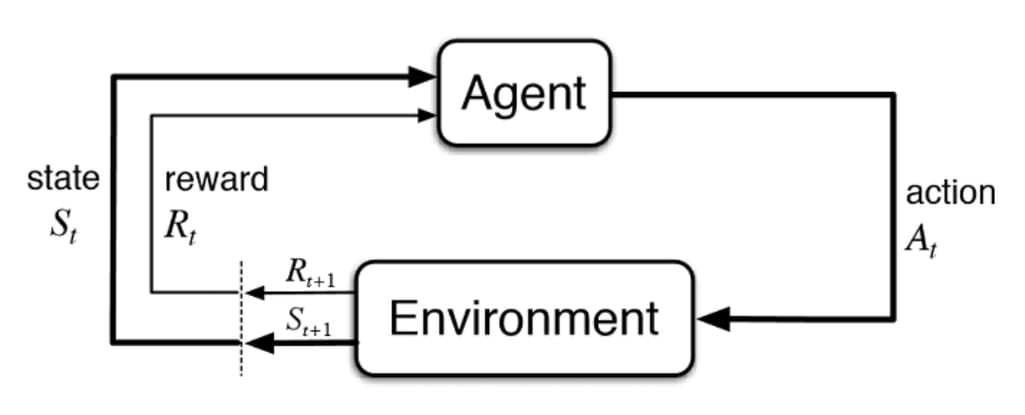
\includegraphics[width=10cm]{images/reinforcement_learning_scheme.jpg}
\caption{Reprezentarea vizuală a unui PDM \cite{reinforcement_learning_scheme_image}}
\end{figure}

\subsection{Funcții de valoare și politici optime}
\subsubsection{Funcția de politică a agentului}
În contextul mediului definit, \textbf{politica} (policy) reprezintă "strategia" pe care o urmează agentul în cazul determinării acțiunii potrivite. Aceasta concretizează mecanismul probabilistic parcurs de agent în cadrul unei "rute" de stări.

Aceasta poate fi de două feluri:
\begin{enumerate}
    \item \textbf{Politica deterministă}: $\pi:S \xrightarrow{} A$
    \begin{itemize}
        \item Mapează fiecare acțiune la o singură stare
        \item Exemplu: Când pică bicicleta, o ridic.
    \end{itemize}
    \item \textbf{Politica stocastică}:  $\pi:S \times A \xrightarrow{} [0, 1]$
    \begin{itemize}
        \item Definește o distribuție de probabilitate peste acțiuni pentru fiecare stare
        \item $\pi(a|s)$ = probabilitatea de a alege acțiunea $a$ în starea $s$
        \item Exemplu: Atunci când se murdărește bicicleta, 90\% din timp o voi spăla imediat, iar 10\% din timp o voi curăța a doua zi.
    \end{itemize}
\end{enumerate}

Politicile stocastice permit agentului să exploreze diferite acțiuni ceea ce cresc șansele de descoperire a unei politici optime, care să poată fi exploatată ulterior. Totodată, ele conferă și robustețe făcând predicția comportamentului mai puțin anticipabilă de către adversari.

\subsection{Evaluarea politicilor: Funcțiile de valoare}
Pentru a determina cât de bună este o anumită politică, avem nevoie de o modalitate de măsură a performanței acesteia. Cu ajutorul funcțiilor de valoare, putem defini o metrică ce estimează gradul de utilitate al unei situații sau acțiuni raportat la ajutorul oferit atingerii scopului predefinit.

Va trebui mai întâi să definim noțiunea de \textbf{episod}, care reprezintă secvența ordonată temporal al tuplurilor de acțiune și stare, pe care agentul o întreprinde pornind de la o stare inițială până la o stare terminală, $t$.
\begin{center}
    $s_0a_0, s_1a_1, \space ..., s_ta_t$
\end{center}

Funcția de valoare a stării (State Value Function) $V^\pi(s)$ reprezintă recompensa totală așteptată pe care o poate obține agentul pornind din starea $s$ și urmând politica $\pi$ pentru tot restul episodului.
\begin{center}
    $V^\pi(s) = E_\pi[\sum_{t=0}^\infty \gamma^t R_{t+1} | S_0 = s]$, unde:
\end{center}
\begin{itemize}
    \item \textbf{$E_\pi$} este valoarea așteptată, urmărind politica $\pi$
    \item \textbf{$\gamma ^ t$} este factorul de discount aplicat recompensei de la timpul $t$
    \item \textbf{$R_{t+1}$} este recompensa primită la timpul t+1
    \item \textbf{$S_0 = s$} este condiționarea că începem din starea $s$.
\end{itemize}

Scrierea extinsă a lui $V^\pi(s)$ ne arată de fapt că acesta doar urmărește care este rezultatul final al deciziilor noastre. Factorul $\gamma$ ne ajută să valorificăm mai mult recompensele imediate, în detrimentul celor viitoare, în practică acesta are o valoare cuprinsă între 0.99 și 0.95, depinzând de context.
\begin{center}
    $E_\pi[R + R\gamma + R\gamma^2 + \space ...]$
\end{center}

Funcția de valoare acțiune-stare (Action-Value Function/Q-Function) reprezintă recompensa totală așteptată prin luarea acțiunii $a$ în starea $s$, urmată de aplicarea politicii $\pi$ pentru restul episodului.
\begin{center}
    $Q^\pi(s,a) = E_\pi[\sum_{t=0}^\infty γ^t R_{t+1} | S_0 = s, A_0 = a]$, unde:
\end{center}
\begin{itemize}
    \item la fel ca mai sus, regăsim aceiași termeni, doar că vom condiționă acum utilizarea acțiunii $a$ în starea $s$ prin $S_0 = s, A_0 = a$.
\end{itemize}

Diferența dintre cele două este că funcția $Q$ ne permite să alegem ce acțiune să fie utilizată prima dată, după care ambele funcții urmăresc evoluția evenimentelor alese prin politica $\pi$. În practică preferăm să utilizăm funcția $Q$ deoarece ne permite să alegem cea mai bună acțiune într-o stare, astfel ajungând la un rezultat optim. Relația dintre cele două este că funcția de valoare $V$ este media ponderată după probabilitate de a acționa în starea $s$ cu acțiunea $a$, conform cu funcția $Q$:
\begin{center}
    $V^\pi(s) = \sum_a \pi(a|s) Q^\pi(s,a)$
\end{center}

\subsection{Ecuația Bellman: Principiul optimizării dinamice}
Ecuația Bellman este cea mai importantă relație matematică oferind o modalitate de a exprima valorile în termeni recursivi. Ecuația spune că valoarea unei stări (sau a unei combinații de stare-acțiune) este egală cu recompensa imediată așteptată plus valoarea ponderată de discount al situației următoare.

\begin{equation}
V^\pi(s) = \sum_a \pi(a|s) \sum_{s'} P(s'|s,a)[R(s,a,s') + \gamma V^\pi(s')]
\label{eq:bellman_v}
\end{equation}

\begin{equation}
Q^\pi(s,a) = \sum_{s'} P(s'|s,a)[R(s,a,s') + \gamma \sum_{a'} \pi(a'|s') Q^\pi(s',a')]
\label{eq:bellman_q}
\end{equation}

\subsection{Politici optime}
Politica optimă $\pi^*$ este cea care maximizează valoarea așteptată pentru toate stările posibile.

\begin{equation}
    \pi^* = \arg\max_\pi V^\pi(s) \text{ pentru toate } s \in S
\label{eq:optim_pi}
\end{equation}

Pentru orice proces de decizie Markov finit, există cel puțin o politică optimă deterministă $\pi^*$. Deși pot exista mai multe politici optime, funcția de valoare optimă $V^*(s)$ este unică pentru fiecare stare $s$, toate politicile optime având aceeași funcție de valoare $V^*(s) = V^{\pi^*}(s)$.

Utilizând rezultatele de mai sus \ref{eq:bellman_q}, \ref{eq:bellman_v}, \ref{eq:optim_pi}, putem construi ecuațiile Bellman pentru politica optimă:
\begin{equation}
    V^*(s) = \max_a \sum_{s\prime} P(s\prime|s,a)[R(s,a,s\prime) + \gamma V^*(s\prime)]
\label{eq:bellman_v_optim}
\end{equation}

\begin{equation}
    Q^*(s,a) = \sum_{s\prime} P(s\prime|s,a)[R(s,a,s\prime) + \gamma \max_{a\prime} Q^*(s\prime,a\prime)]
\label{bellman_q_optim}
\end{equation}

Astfel, conform \ref{bellman_q_optim} și \ref{eq:bellman_v_optim} putem extrage politica optimă cu ajutorul funcției $Q$ optime, un rezultat foarte important pentru progresul curentei lucrări. Odată determinată funcția $Q$ optimă $Q^*(s, a)$, obținerea politicii optime devine trivială, alegând mereu cea mai mare valoare a funcției $Q$ în fiecare stare.

\begin{equation*}
    \pi^*(s) = \arg\max_a Q^*(s,a)
\end{equation*}
\chapter{Modelarea jocului}

\section{Bazele jocului Monopoly}
\subsection{Elementele jocului}
Jocul Monopoly se bazează pe concurența jucătorilor cu scopul stabilirii unui monopol capitalist în speranța obținerii unui venit pasiv stabil și profitabil. Acesta se bazează pe elemente stocastice precum aruncarea zarurilor și cartonașele „Cufărul Comunității" și a celor „Șansa" pentru a încerca să uniformizeze cât mai mult șansa de câștig.

Monopoly dispune de o tablă divizată în 40 de căsuțe, subdivizate în 5 categorii, pe baza rolului acestora în joc. De asemenea acesta mai beneficiază și de elemente adiacente ce contribuie la complexitatea și deciziile luate:

\begin{itemize}
    \item \textbf{Proprietățile imobiliare}: Sunt zonele cumpărabile ce simbolizează un cartier, zonă sau bulevard din lumea reală, grupate după o culoare ce reprezintă aprecierea acestora. Jucătorii se întrecu în cumpărarea acestora, urmând ca apoi orice alt jucător ce nu deține proprietatea să fie considerat un chiriaș, fiind nevoit să plătească chirie proprietarului.
    \item \textbf{Case și hoteluri}: Sunt modalități de îmbunătățire a venitului pasiv și consolidării monopolului deținut. Odată deținute toate proprietățile de aceeași culoare, se consideră că jucătorul deține monopol pe culoarea respectivă, acesta putând amplasa case și hoteluri cu scopul măririi chiriei percepute pe fiecare proprietate.
    \item \textbf{Gările}: Sunt zone cumpărabile, ce se diferențiază prin caracterul lor static (nu pot fi îmbunătățite), dar care contribuie prin incrementarea chiriei percepute pe fiecare unitate, prin numărul lor.
    \item \textbf{Utilitățile}: Sunt zone cumpărabile, statice, ce beneficiază de mărirea chiriei pe baza unui factor de multiplicare în urma aruncării zarurilor. Ca și în cazul gărilor, numărul utilităților deținute, îmbunătățește considerabil chiria percepută.
    \item \textbf{Șansa și Cufărul Comunității}: Sunt căsuțe ce necesită extragerea unui cartonaș din teancul corespunzător și executarea acțiunii imediat al acestuia.
    \item \textbf{Cartonașele Șansa și Cufărul Comunității}: Acestea ascund atât evenimente negative, precum plătirea unui impozit, cât și evenimente neutre sau ajutătoare.
    \item \textbf{Căsuțele Taxă}: Sunt căsuțe ce necesită plata imediată a unei sume afișate.
    \item \textbf{Căsuțele din colțuri}: Sunt elemente definitorii pentru joc, ele având diferite acțiuni.
    \item \textbf{Banii}: Sunt resursele cu care jucătorii interacționează cu mediul, folosindu-i pentru a cumpăra sau finaliza acțiuni.
\end{itemize}

\begin{figure}[H]
    \centering
    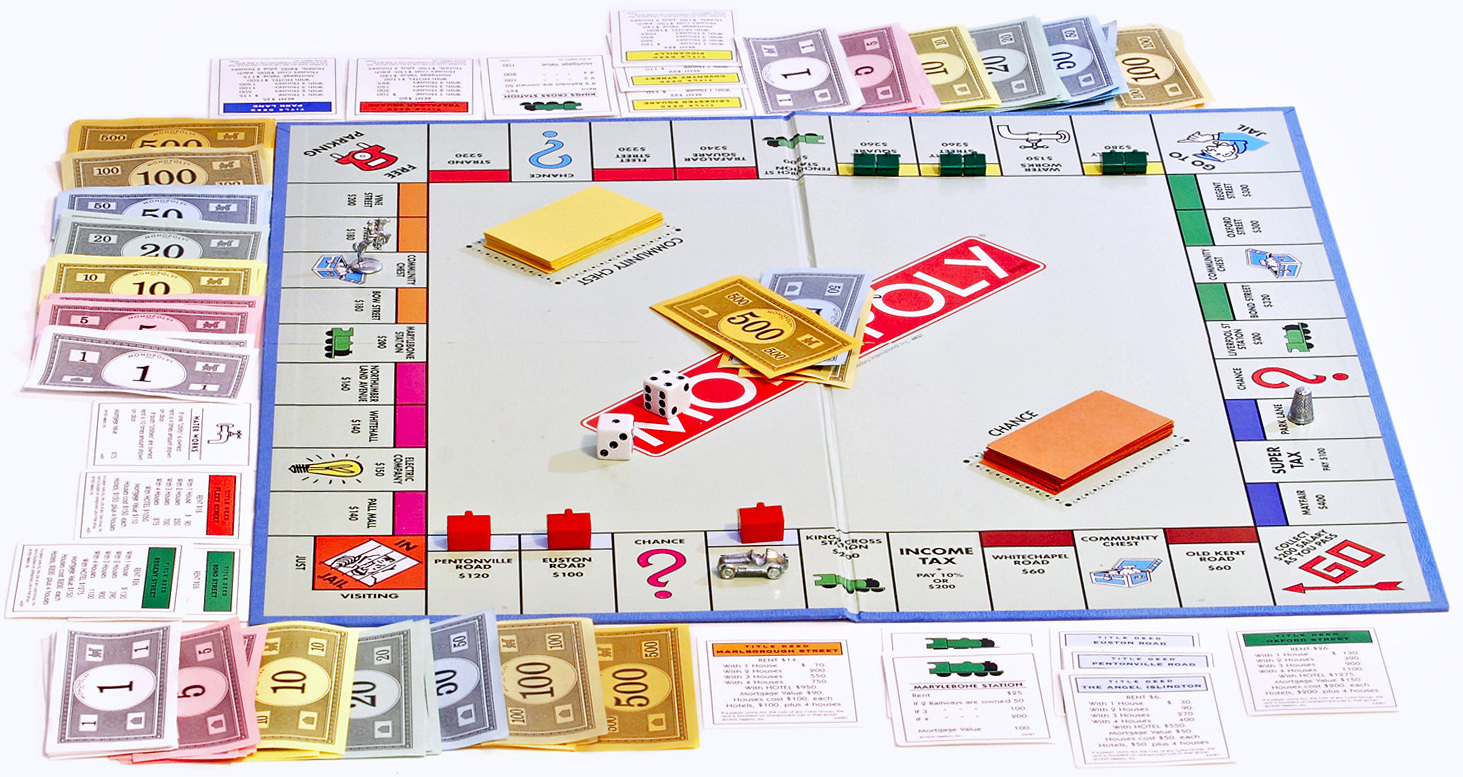
\includegraphics[width=10cm]{images/monopoly_elements.jpg}
    \caption{Elementele disponibile în jocul Monopoly \cite{wikipedia_monopoly}}
    \label{fig:monopoly-elements}
\end{figure}

\subsection{Regulile jocului}
Conform regulilor oficiale \cite{monopoly_rules}, jocul este conceput pentru a fi jucat de 2-4 jucători. Fiecare jucător dispune de un pion și primește o sumă inițială de 1500₩ (simbolul specific al banilor monopoly \cite{monopoly_money}). Jucătorul cel mai tânăr își începe aruncarea zarurilor după își continuă acțiuniile în funcție de căsuța în care a ajuns, rândul său încheindu-se și fiind pasat următorului jucător ca vârstă. Printre acțiunile posibile amintim de: cumpărarea unei proprietăți, licitație pentru o proprietate, cumpărarea unei case, etc. Ordinea definirii acțiunilor și posibilitatea executării lor sunt redate într-o formă sumară în diagrama stărilor din joc \ref{fig:monopoly-rules-state-machine}.

\begin{figure}[H]
    \centering
    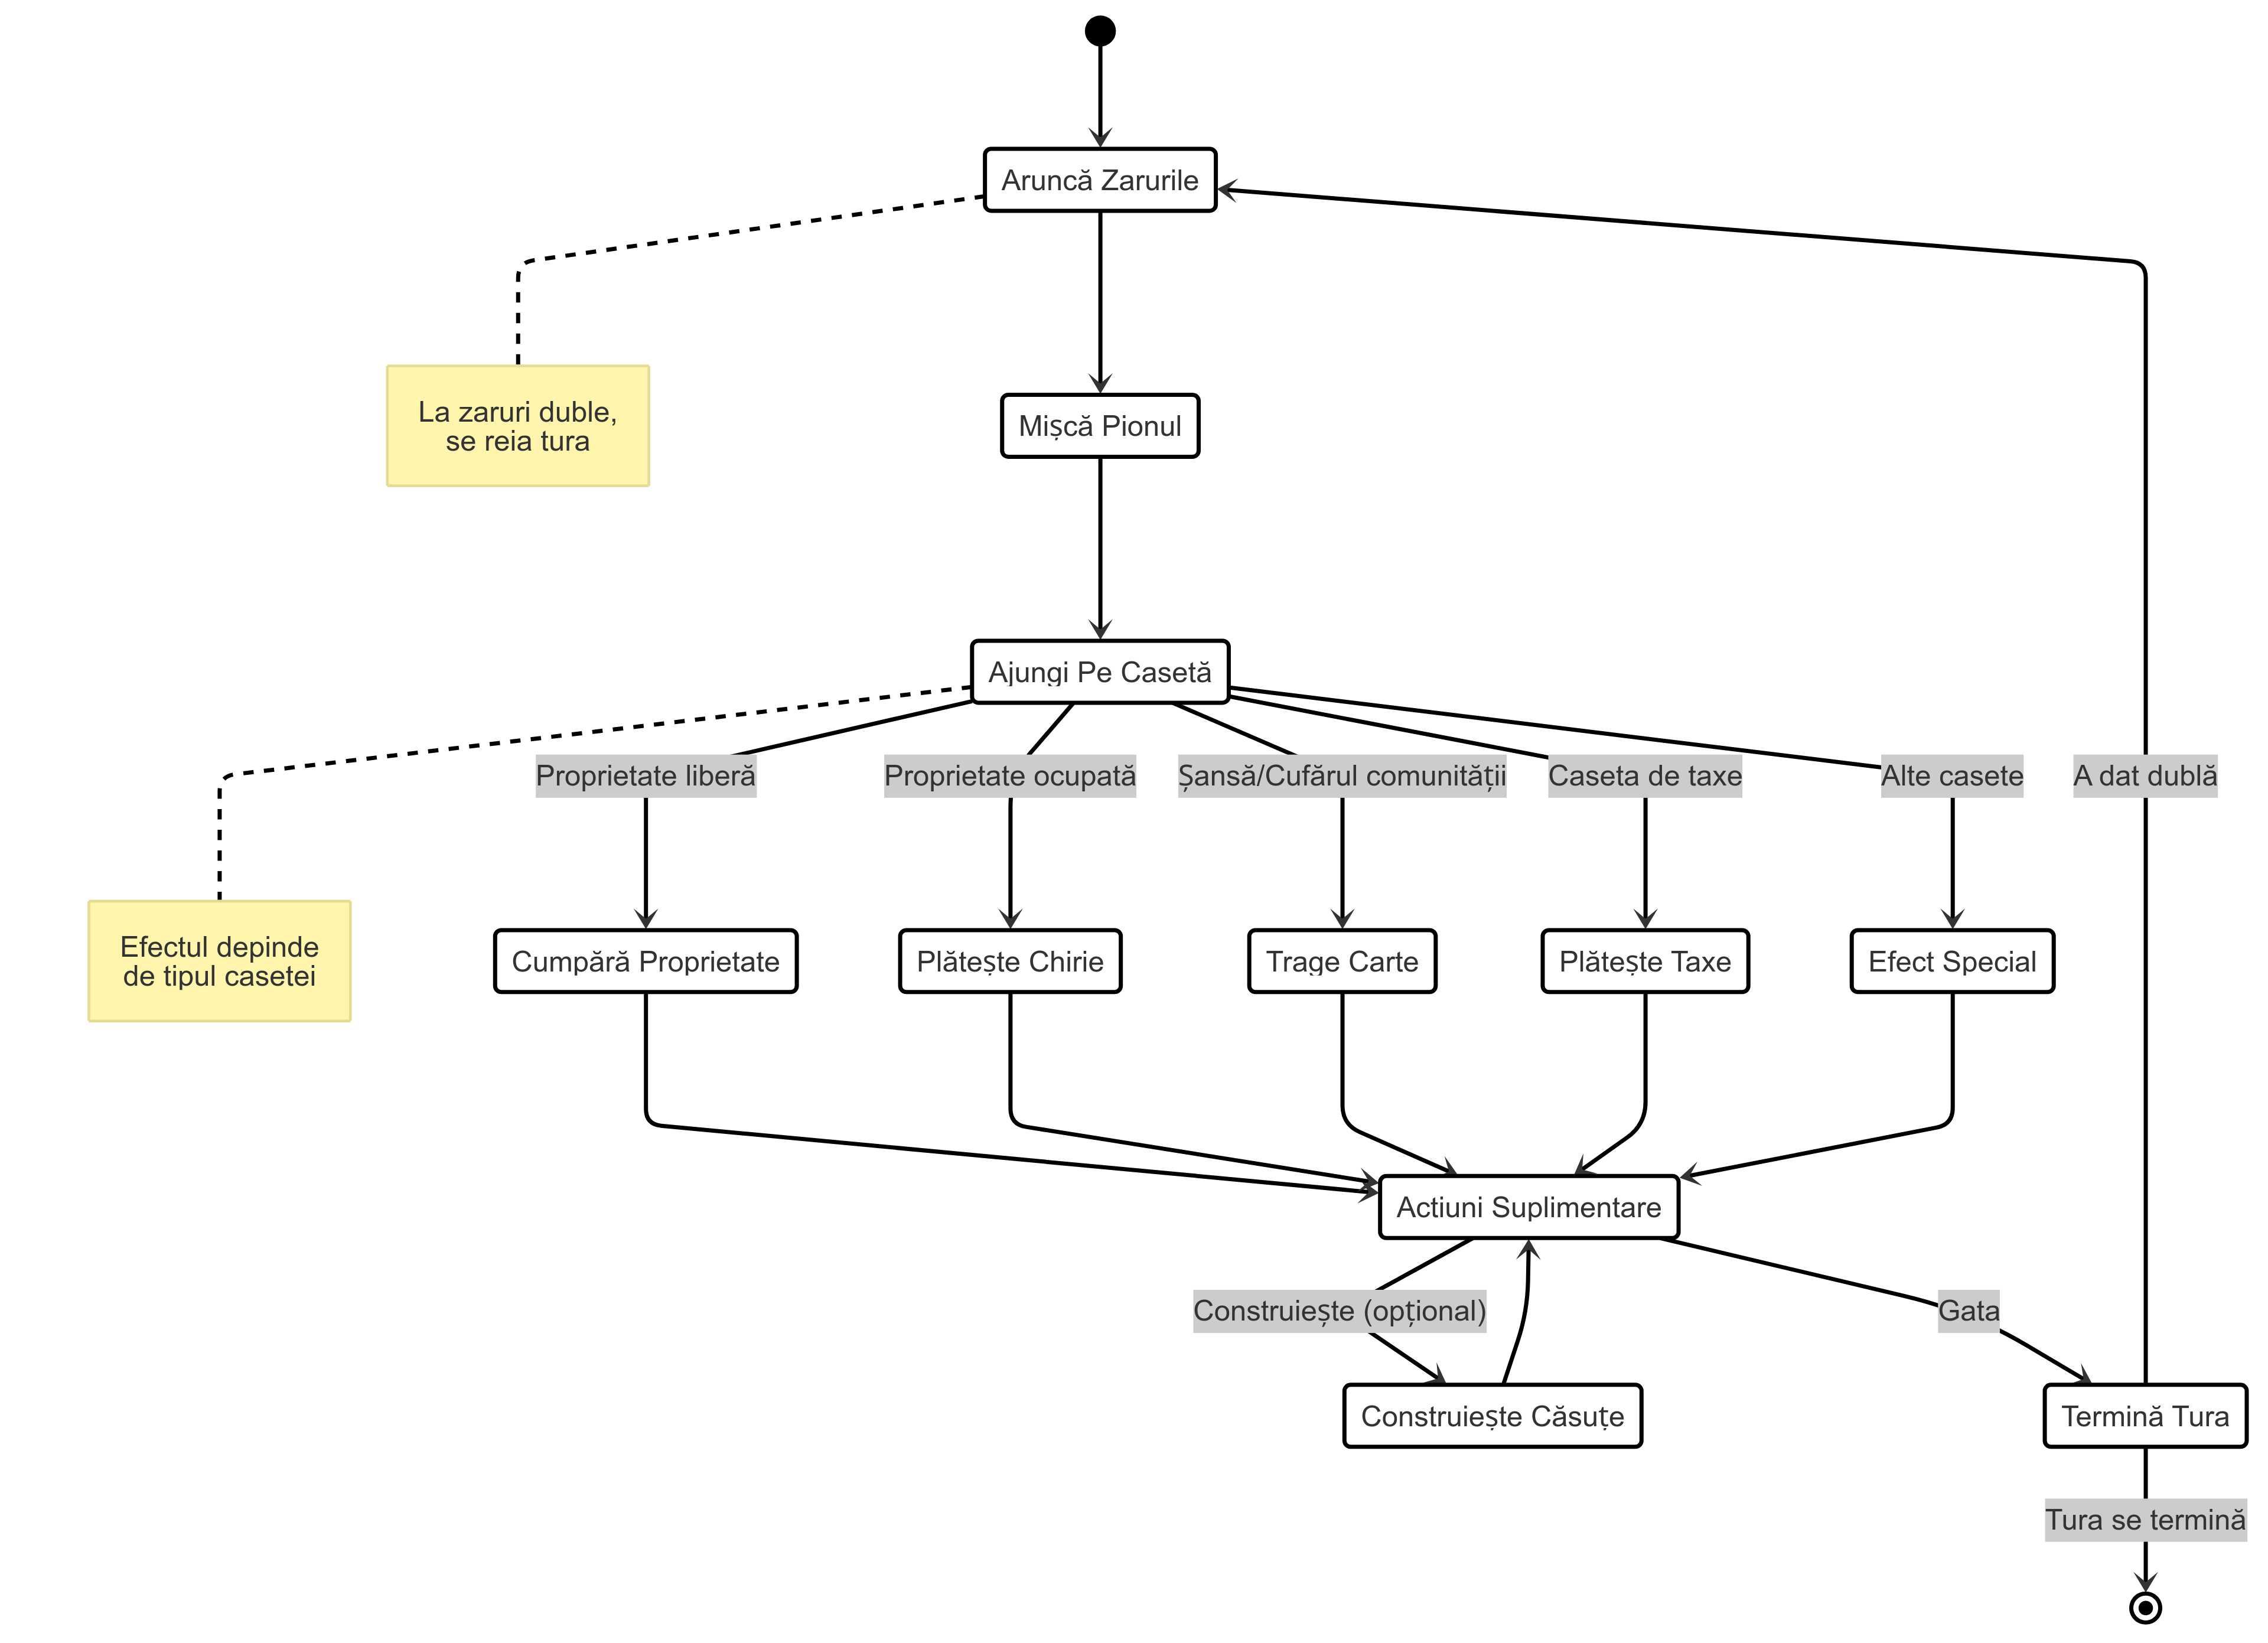
\includegraphics[width=10cm]{images/monopoly_rules_state_machine.png}
    \caption{Diagrama stărilor de joc și a acțiunilor posibile în Monopoly}
    \label{fig:monopoly-rules-state-machine}
\end{figure}

\subsection{Scopul jocului}
Fiecare jucător adună proprietăți, monopoluri, case și hoteluri de-a lungul unui episod. Scopul jocului este ca averea colectată din toate sursele, inclusiv banii cash, să fie cea mai mare. Decizia de încetare a jocului poate fi unanimă, moment în care fiecare jucător își calculează averea și se face poziționarea în clasament. Pe parcursul derulării jocului, dacă un jucător nu își poate plăti datoria, acesta este declarat falimentar și părăsește jocul. Ultimul jucător în joc este, de asemenea, considerat câștigător.

\section{Adaptări pentru reinforcement learning}
Datorită mediului digital și determinist ce constrânge implementarea realistă a jocului, câteva modificări vor trebui făcute pentru ușurarea atât a reprezentării cât și a redării fidele a unei reprize de joc.

Trebuie precizat că în ciuda intuiției naturale, anumiți factori de mediu pot influența dramatic buna desfășurare și simulare a jocului. Fiind un joc stocastic, bazat pe probabilitatea zarului, o statistică amănunțită \cite{monopoly_statistics} ne arată clar că nu toate proprietățile sunt uniform distribuite în cazul frecvenței vizitării lor. Acest lucru este de așteptat având în vedere distribuția probabilistică a zarurilor ce favorizează apariția numerelor 6, 7, 8 \cite{dice_statistics}.

Distribuția neuniformă poate influența și deciziile jucătorilor în estimarea venitului optim. Aceasta impune ca anumite proprietăți vor fi frecventate mai des decât altele \cite{monopoly_statistics_positions}, astfel impunându-se un factor bias în deciziile jucătorilor. Bazat pe frecvența vizitelor, se poate constata că o preponderență vizitare a culorii portocalii și a celei roșii ar aduce cel mai bun randament. Acest raționament se bazează pe ajungerea frecventă la închisoare, din multiple motive, iar distribuția neuniformă favorizând vizitarea căsuțelor corespunzătoare culorilor amintite, în urma ieșirii din închisoare.

Un alt lucru observabil este diminuarea realizărilor de monopoluri și uniformitatea jocului în cazul participării a mai mult de 2 jucători \cite{monopoly_statistic_players}. Nu doar că diferența de monopolizare crește, ba mai mult în cazul jocurilor cu mai mulți jucători, se observă clar o diferență în procentajul de câștig al jucătorilor care încep primii, aceasta putând ajunge și la 5\% diferență de procentaj în cazul ratei de câștig.

\subsection{Simplificarea regulilor}
Astfel observând regulile oficiale amintite anterior, dar și prin constatare personală în urma jucării Monopoly, am decis că anumite elemente sau aspecte pot fi reduse, fără a afecta negativ calitatea jocului sau influența rezultatul final.

O prima modificare va fi \textbf{limitarea numărului de jucători} la doar doi. Deși implementarea curentă poate susține un număr de până la 4 jucători, am decis că rezultatele și experimentele derulate să fie restrânse doar la doi jucători, pentru a favoriza dinamicitatea și posibilitatea dezvoltării rapide. Conform mențiunilor anterioare, un mediu cu prea mulți jucători se va baza exclusiv pe realizarea ofertelor de schimb pentru a se putea dezvolta monopoluri și a avea un rezultat final concludent. Mi-am dorit să elimin dependența de factori stocastici cât mai mult și să favorizez buna desfășurare a unui joc convergent către o stare definitivă. Astfel fiecare jucător va putea să își construiască și aplice strategia proprie fără a fi constrâns de factori externi.

O a doua modificare concludentă este \textbf{secvențierea acțiunilor} întreprinse. Dinamicitatea jocului ar fi îngreunat considerabil atât finalitatea unui episod, cât și reprezentarea sa eficientă. Un joc amical în lumea reală se bazează pe posibilitatea de interacțiune permanentă cu mediul chiar și în lipsa turului curent. Orice jucător poate, conform regulilor oficiale, să își îmbunătățească proprietățile, întreprindă schimburi, ipotecheze proprietăți, etc. în afara turului său. Decizia de urma modelarea conform standardelor actuale ar fi condus la o lipsă de convergență rapidă și o durată îndelungată a unui episod pentru a putea conchide asupra câștigătorului. Deși restricționează ferm acțiunile întreprinse, această modificare nu subvine în scopul schimbării interacțiunii, ci este doar o constrângere benefică în planificarea și consolidarea unui mecanism clar de acționare, defavorizând decizii spontane și adesea haotice. O bună detaliare asupra acestei secvențieri va fi detaliată în continuare.

Pe lângă modificările de mediu definitorii de mai sus, amintim și alte abăteri de la regulile oficiale cu scopul unei modelări mai agreabile ale environment-ului:
\begin{enumerate}
    \item \textbf{Procesul de licitație}: În regulile oficiale, în urma refuzului de achiziționare a unei proprietăți, aceasta trebuie supusă unei licitații, în care pot participa toți jucătorii, inclusiv cel care a refuzat. În urma unei analize, având la dispoziție doar doi jucători, procesul de cumpărare al unei proprietăți s-ar fi complicat linear, astfel am decis că achiziționarea unei proprietăți să fie o decizie binară cu putere de influențare nulă în exterior. Jucătorul care a ajuns pe proprietatea după mutare, poate fie să o cumpere, în cazul existenței fondurilor disponibile, fie să o refuze, astfel proprietatea rămânând în posesia băncii.
    \item \textbf{Dezvoltarea proprietăților}: Se face deodată, pentru întreg grupul de culoare, spre deosebire de regula standard, unde se poate face individual per proprietate. Această schimbare s-a făcut prin prisma constrângerii deciziei de investire cu planificare pe timp lung. Îmbunătățirea proprietăților ar trebui să fie o decizie importantă și un considerent major, nu doar o acțiune efectuată. Astfel prin această restrângere, fiecare jucător va trebui să cântărească atent decizia de a investi mai mulți bani deodată, cu promisiunea unui retur viitor al investițiilor.
    \item \textbf{Ignorarea limitelor resurselor}: Jocul oficial presupune existența unor resurse fizice limitate, precum bancnotele și casele/hotelurile. Am făcut abstracție de această limitare, dorind să ofer posibilitatea desfășurării strategiei optime. Într-adevăr, limitarea numărului de case și dispunerea acestora în urma unei licitații, ar fi crescut competitivitatea și previziunea jucătorilor, dar în același timp ar fi adăugat informație în plus de gestionat și îngreunat procesul simulării.
    \item \textbf{Dobânda proprietăților ipotecate}: Regulile curente ale jocului, privind plata unei dobânzi și ale unei sume adiționale în cazul ridicării ipotecii de pe o proprietate erau puțin complicate și de un interes scăzut. Astfel am decis că această regulă să fie ignorată și ridicarea ipotecii să poată fi făcută doar de jucătorul care a ipotecat-o, plătind cei 10\% din valoare proprietății.
    \item \textbf{Taxa pe venit}: Atunci când jucătorul ajunge pe căsuța "Taxa pe venit" are posibilitatea să plătească o sumă statică de 200₩ sau poate opta pentru plata a 10\% din totalul deținut, decizia trebuind luată fără a calcula cât reprezintă totalul deținut. Din cauza digitalizării jocului, această decizie ar fi fost trivială, totalul deținut fiind automat calculat și cunoscându-se de-a lungul jocului, fapt pentru care se va plăti constant suma de 200₩.
    \item \textbf{Sistemul de faliment}: Când un jucător nu își poate plăti o chirie, taxă sau orice sumă datorată, acesta este obligat să vândă ce are în scopul achitării datoriei, avand o singura sansa de redresare per actiune intreprinsa. În cazul în care nu reușește să strângă valoarea necesară, acesta este declarat "în faliment" (bankruptcy) și toată averea sa este împărțită în mod echitabil fiecărui jucător. În cazul nostru, având doar doi jucători, jocul se va termina iar jucătorul cu cea mai mare avere va fi declarat câștigător. De remarcat totuși, că implementarea oferă suport pentru a decide o alternativă a finalității jocului.
\end{enumerate}

\section{Arhitectura Generală a Sistemului}

\subsection{Principii de design}
În vederea construirii unui sistem reprezentativ, fidel și scalabil de simulare va trebui să avem în vedere separarea atribuțiilor și responsabilităților. Simulatorul nostru va trebui să mențină constant o stare a jocului cât mai fidelă de un joc real, asigurându-se constant că starea curentă și acțiunile efectuate respectă regulile impuse. De asemenea, acesta va trebui să permită adăugarea și modificarea jucătorilor folosind o metodă eficientă și va trebui să se asigure de coordonarea și secvențierea acțiunilor.

Mai mult de atât, va trebui să avem în vedere și nevoia simulării unui număr mare de jocuri, ceea ce ne constrânge să optimizăm sistemul și să ne asigurăm că acesta va funcționa fără probleme sub stres. Elementele sale trebuie să fie paralelizabile pentru a putea atât antrena cât și simula pe un număr cât mai mare de date într-un interval temporal predefinit.

\begin{figure}[H]
    \centering
    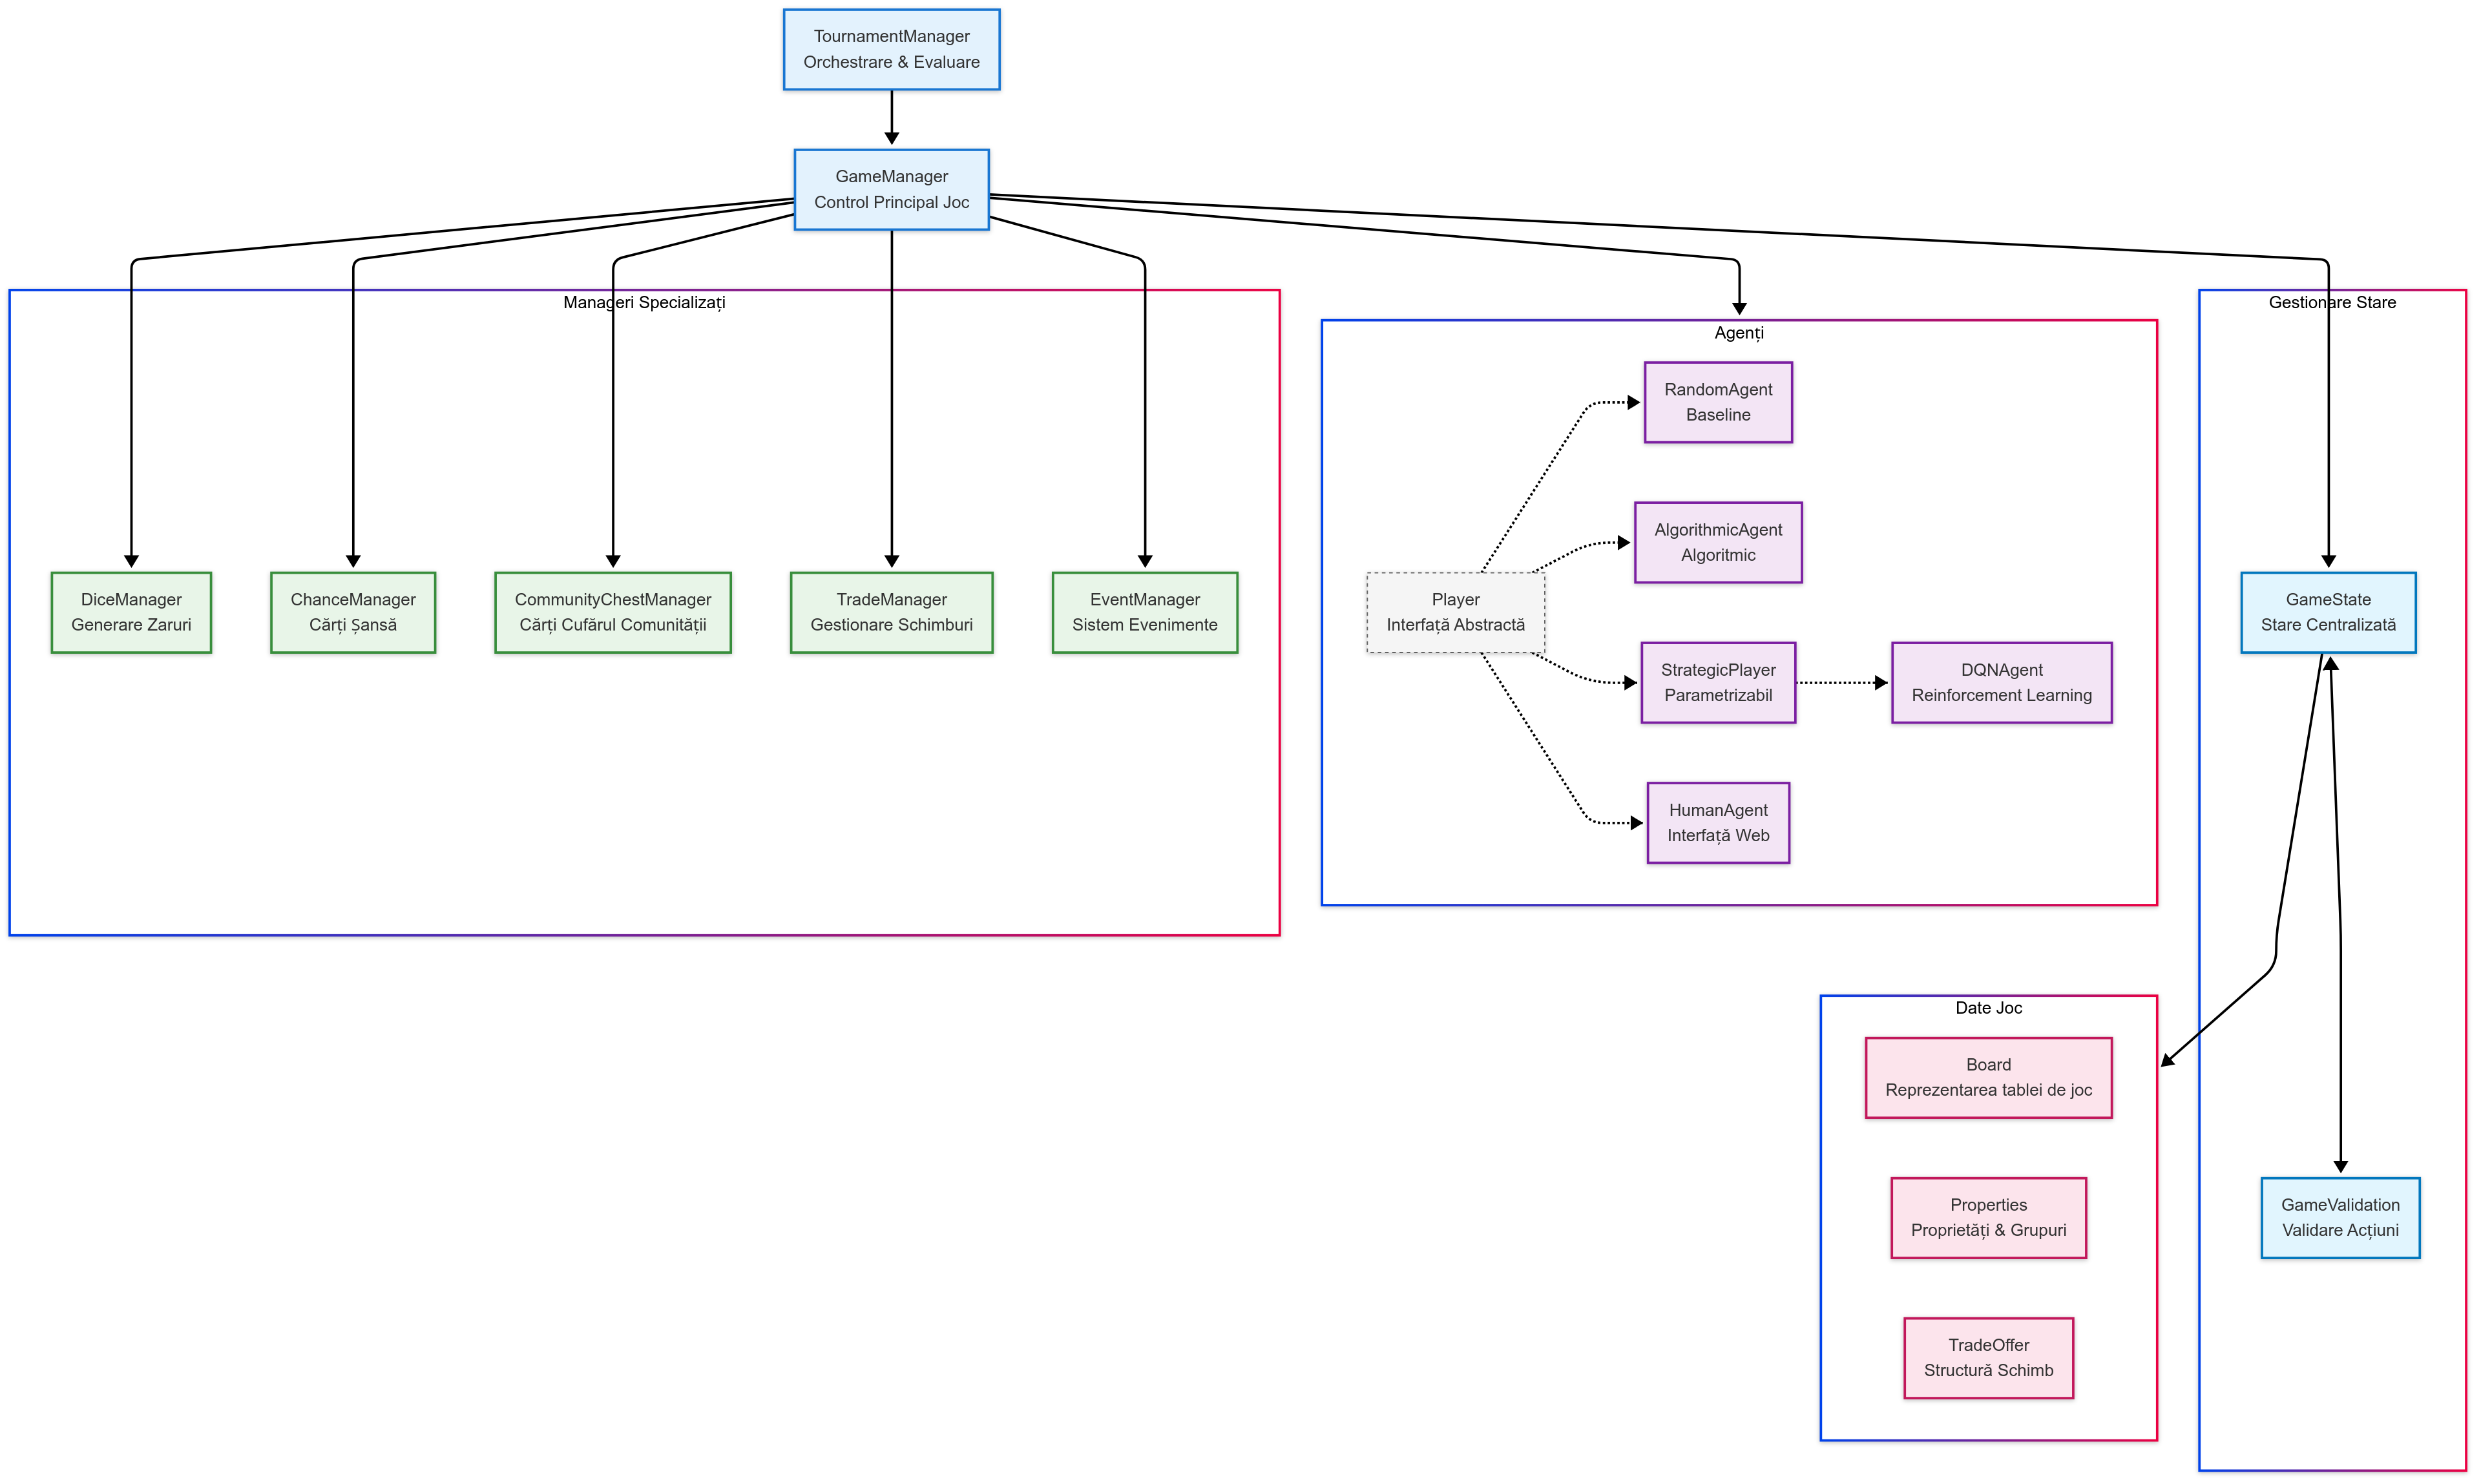
\includegraphics[width=15cm]{images/diagrama_flow.png}
    \caption{Diagrama arhitecturii generale a sistemului}
    \label{fig:diagrama-responsabilitati}
\end{figure}

\subsection{Separarea responsabilităților}
Delimitarea și îngrădirea răspunderii reprezintă un principiu de proiectare și arhitectură des întâlnit în lumea programării. Principiul responsabilității singulare (Principal of Singular Responsabilities) \cite{srp_desing_pattern}, face parte din familia principiilor SOLID \cite{solid_patterns} și favorizează scalabilitatea prin minimizarea funcționalităților unei entități. Minimizarea face ca testarea să fie mai unitară, iar dependințele mai puține, astfel crescând organizarea și lizibilitatea codului.

Menținerea principiului este evidențiată prin izolarea a trei componente importante în sistemul proiectat ce conlucrează împreună și se asigură de buna funcționare a simulării, conforme cu teorema:

\begin{displayquote}
\centering
\textit{Adună împreună lucrurile care se schimbă din aceleași motive. \\
Separă lucrurile care se schimbă din motive diferite.} \cite{srp_quote_source}
\end{displayquote}

Cele trei componente definitorii sunt:
\begin{itemize}
    \item \textbf{Sursa de adevăr}: Cea care se ocupă de menținerea constantă a reprezentării interne și fidele a jocului în orice moment de timp. Aceasta este singura ca poate modifica intern, în urma validărilor, starea jocului, la cerere din exterior și să se asigure că nu există probleme de integritate a datelor.
    \item \textbf{Orchestratorul central}: Cel care se ocupă de secvențierea acțiunilor, de derularea și simularea corectă a jocului, de interacțiunea dintre toate componentele, asigurând o bună funcționare a sistemului.
    \item \textbf{Jucătorii}: Cei care interacționează direct și produc schimbări în mediu, acționând voit printr-o politică internă cu scopul de a perturba și influența rezultatul jocului.
\end{itemize}

Pe lângă componentele principale enunțate anterior, se regăsesc și subcomponente ce preiau din atribuțiile părintelui și le segmentează în acțiuni atomice grupate. Acestea nu sunt decât niște extensii specializate, menite să ușureze și mai mult conceptualizarea reprezentării și ajutând cu evidențierea directă a nevoilor sistemului.

\subsection{Componentele sistemului}
Proiectarea arhitecturală anterioară ne oferă o bază bună de plecare în gândirea structurală a sistemului de simulare. Raportându-ne la aceasta putem implementa efectiv la nivel de cod toate noțiunile discutate anterior.

Datorită simplității, a folosirii sale pe scară largă, atât în domeniul cercetării, cât și în producerea de produse software, dar și a suportului vast, am preferat să folosesc ca și limbaj de programare Python \cite{python_org}. Acesta oferă suport pentru consolidarea structurilor și interacțiunilor prin clase, folosind paradigma de programare orientată pe obiecte \cite{geeksforgeeks_oops}.

În continuare vom reda principalele componente reprezentate sub forma de clase în codul nostru și vom explica importanța, responsabilitatea și câteva aspecte privind implementarea acolo unde cazul o va cere.

\subsubsection{Componentele de bază}
\subparagraph{GameState(starea jocului)}\label{game-state}
Reprezintă unica sursă de adevăr care încorporează toată informația regăsită într-un joc clasic de Monopoly, precum: poziția jucătorilor, jucătorul curent, banii fiecărui jucător, proprietățile deținute, etc. Acesta are la bază o subentitate a tablei de joc ce are ca scop oferirea informațiilor privind costul unei proprietăți, număr de entități dintr-o grupă de culoare, cât și alte informații utile în determinarea informațiilor privind tabla și cartonașele de joc.

Clasa este responsabilă de actualizarea atomică a fiecărei componente la cerere, prin intermediul unor metode predefinite. În caz de eroare, acesta o va propaga mai departe, neintrand în responsabilitatea sa tratarea erorilor.
\subparagraph{GameValidation(validarea jocului)}
O instanță de tip singleton \cite{geeksforgeeks_singleton} ce are drept scop asigurarea respectării integrării cu regulile jocului. Acesta expune metode de verificare ce semnalează prin returnarea unei erori, în cazul producerii uneia. Aici se definesc toate constrângerile necesare efectuării unei acțiuni.
\subparagraph{GameManager(coordonatorul jocului)}
Este orchestratorul principal asigurându-se că toate componentele principale și adiacente se comportă în modul așteptat. La bază acesta expune o metodă pentru simularea unui joc de Monopoly, pentru o stare de joc predefinită.

El creează succesiunea logică de acțiuni ce le întreprinde fiecare jucător la momentul rândului său, asigurându-se că jocul nu s-a terminat și nicio eroare nu a fost întâmpinată. Tratarea erorilor se va face din exterior, acesta doar propagându-le mai departe.

Gestionarea tuturor resurselor auxiliare, precum zarurilor, cartonașelor, etc., este făcută cu ajutor componentelor auxiliare. Acestea expun metode utilizate de clasa coordonatoare cu scopul determinării și întreprinderii acțiunii corespunzătoare.

O reprezentare detaliată a tranzițiilor în timpul unei ture a unui jucător va fi regăsită în anexă, aceasta necesând o explicație detaliată și o ilustrare complicată. Totuși, pentru o vizualizare rapidă și o înțelegere mai bună a modelării secvențiale a acțiunilor putem să observăm figura \ref{fig:monopoly-rules-state-machine}.

\subsubsection{Componentele auxiliare}
\subparagraph{DiceManager}
Se ocupă de generarea aleatoare a aruncărilor de zar, asigurându-se că aceasta se face cu o distribuție probabilistică uniformă. Pentru optimizare, din cauza numărului crescut de cerere, aruncările de zar sunt precalculate și stocate (cache-uite) pentru o și mai bună convergență și acuratețe privind probabilitatea.
\subparagraph{TradeManager}
Este actorul principal de întreprindere de schimburi, principala sa caracteristică fiind validarea și execuția schimburilor. Pentru că aceasta poate fi dinamică, atât din punct de vedere al numărului de oferte, cât și al obiectelor tranzacționate, acesta joacă un rol foarte important în asigurarea integrității și autenticității schimbului făcut.
\subparagraph{CommunityChestManager/ ChanceManager}
Sunt doi coordonatori ce împart responsabilitatea pentru categorii diferite de acțiuni, fiecare fiind reprezentativ pentru evenimentul stocastic de tragere a unui cartonaș "Cufărul Comunității", "Șansa" respectiv.

Acestea se asigură că există maxim două cărți de evadarea din pușcărie puse în circulație în același timp, și se ocupă de aranjarea și păstrarea ordinii cartonașelor de joc extrase. Ordinea de extragere și de plasare a cartonașelor respectă structura de coadă (queue) \cite{geeksforgeeks_queue} descrisă de regulile oficiale ale jocului. De asemenea sunt responsabili de definirea și executarea acțiunilor descrise pe cartonașele de joc.
\subparagraph{EventManager}\label{event-manager}
Entitatea de înregistrare și distribuire (broadcasting) ale evenimentelor reprezentative din joc. Acestea sunt înregistrate de alți manageri și partajate către toți jucătorii, prin intermediul unor metode expuse. Aceștia din urmă, jucătorii, pot decide în mod particular cum vor să trateze evenimentele și importanța alocată lor. Utilitatea acestei componente este evidențiată mai ales în folosirea ei în interfața grafică, fiind principala sursă de notificare.
\subparagraph{TournamentManager}\label{trade-manager}
O implementare personalizată a unui turneu între o listă de agenți predefiniți, ce captează informații de referință cu scopul unei analize detaliate asupra politicii și strategiilor aplicate. Acesta dispune și de opțiunea de duel în stilul round-robin \cite{wikipedia_roundrobin}, având numeroare optimizări de paralelizare și multiprocesare pentru accelerarea vitizei de calcul.

\subsubsection{Arhitectura agenților}

\begin{figure}[h]
    \centering
    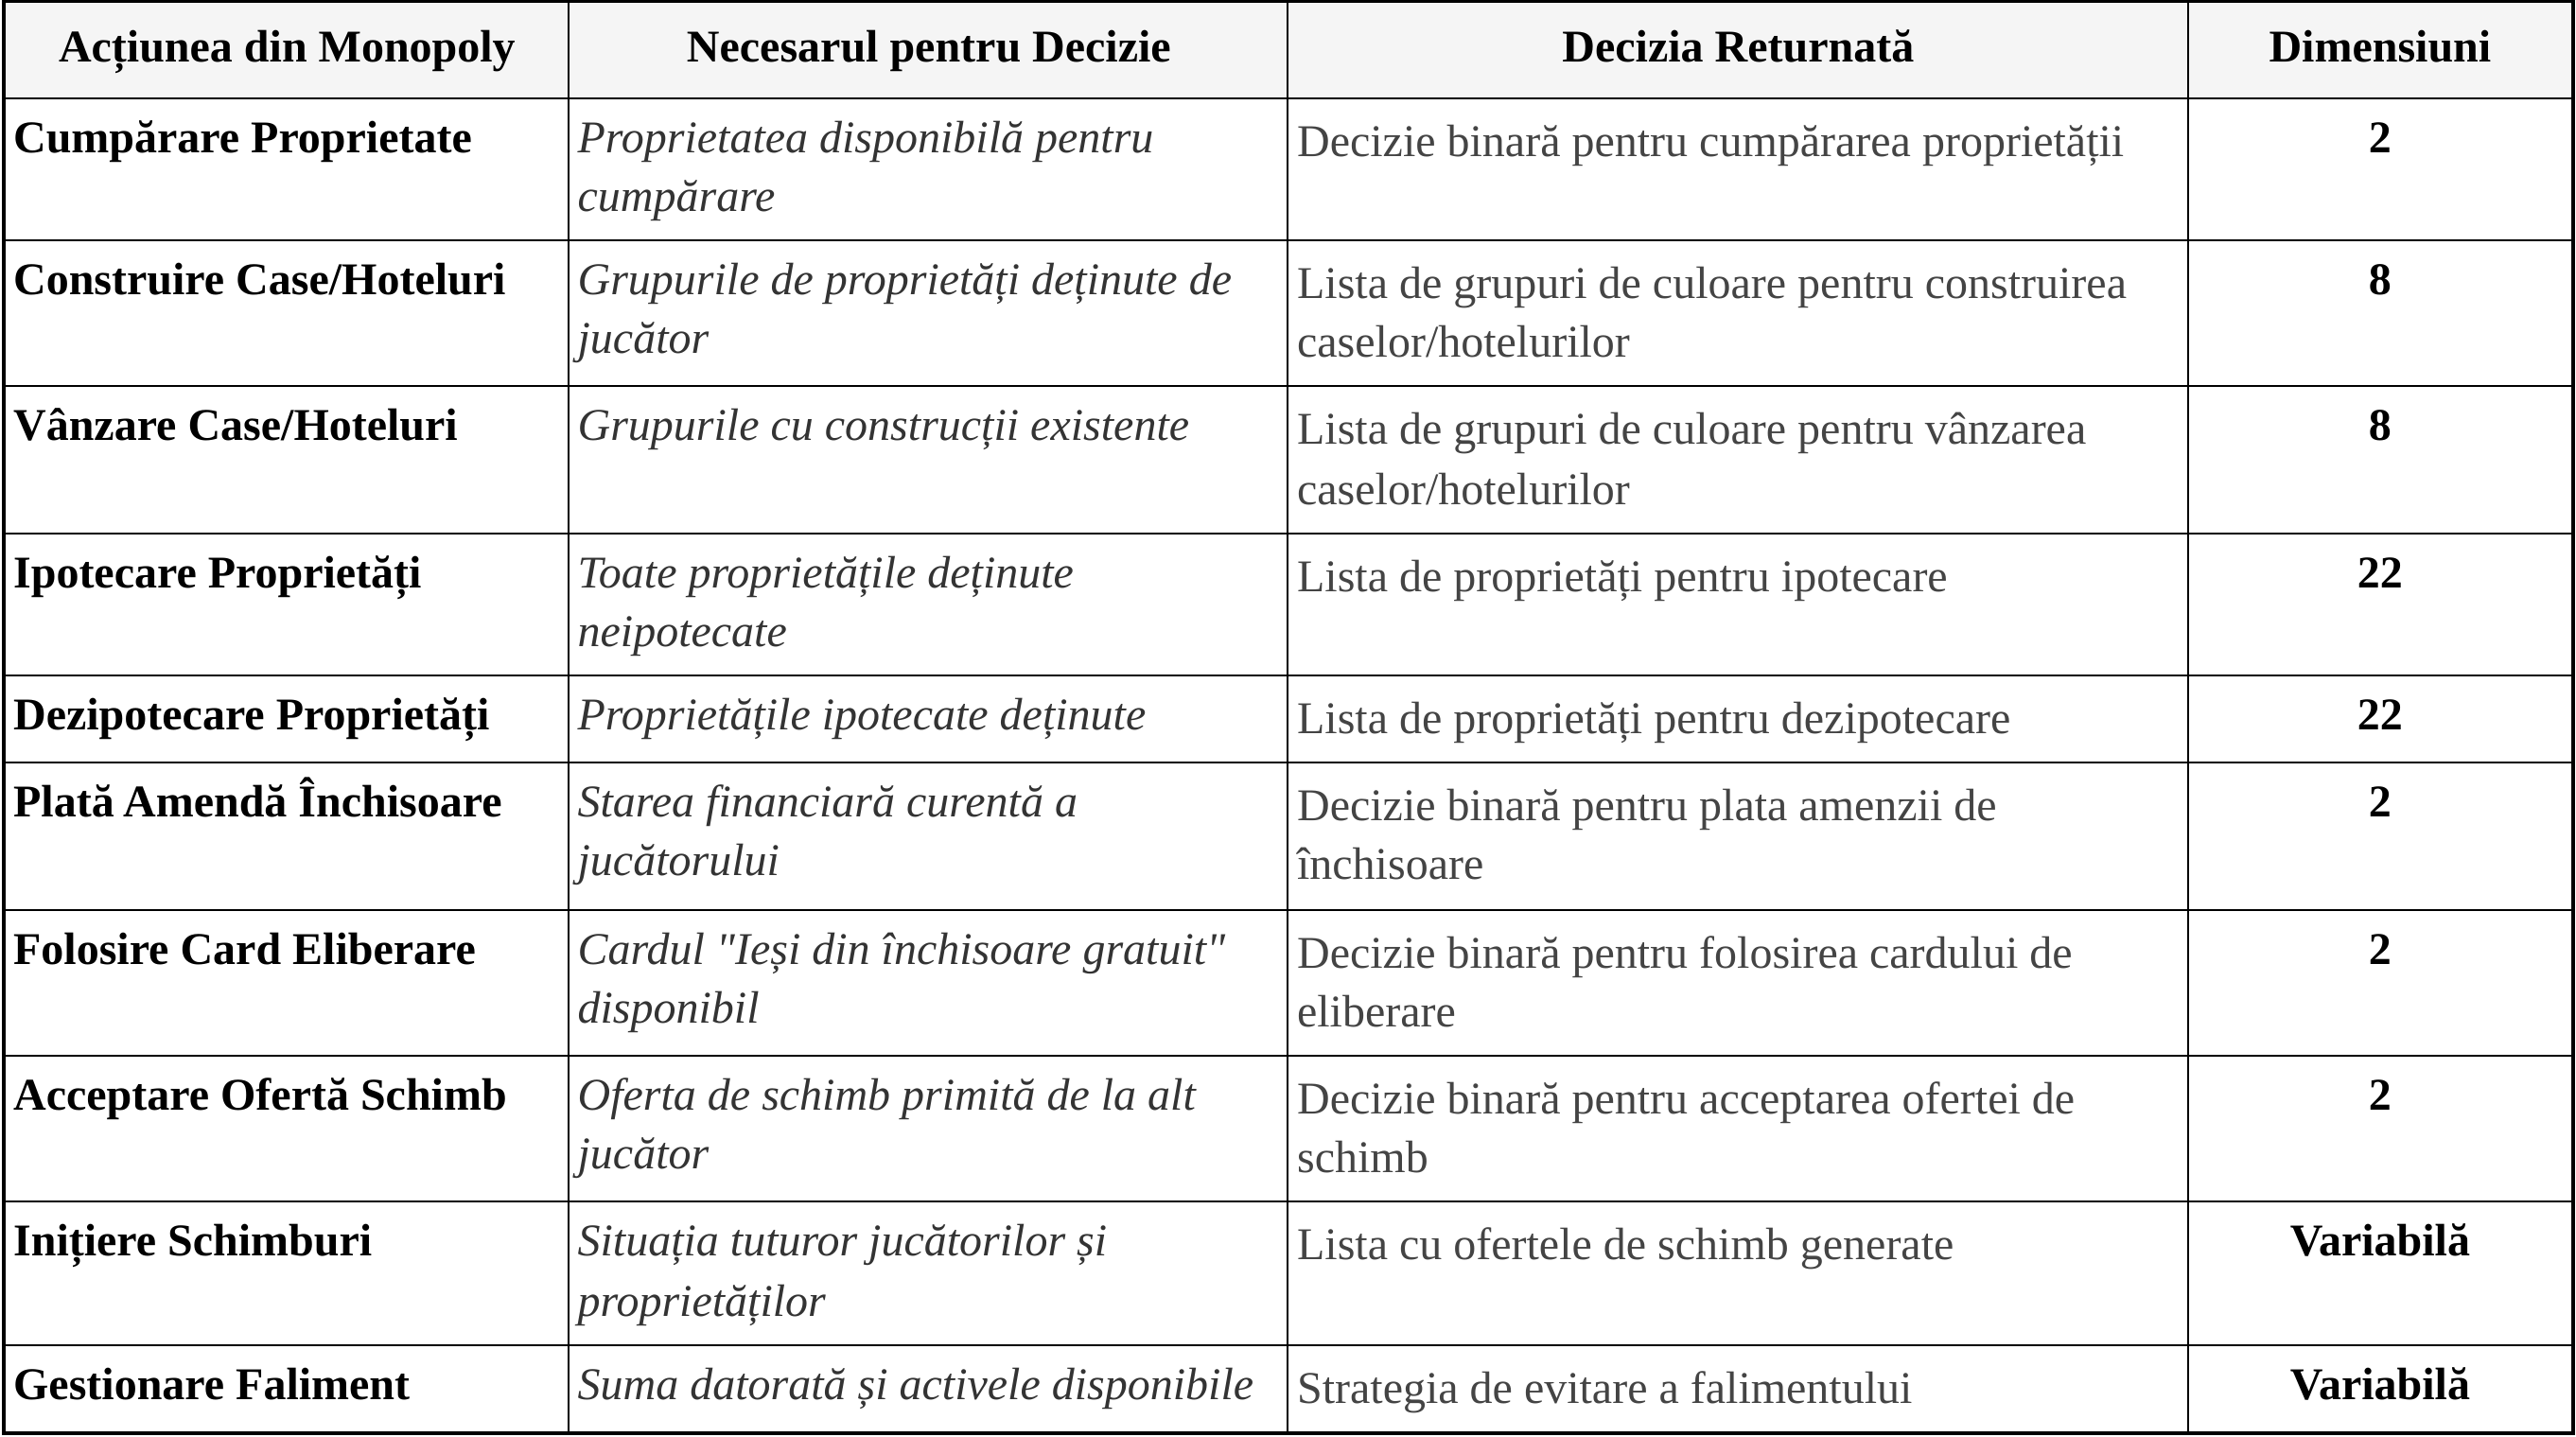
\includegraphics[width=16cm]{images/monopoly_actions_html_table (1).png}
    \caption{Actiunile permise in simulatorul de Monopoly}
    \label{fig:monopoly_actions}
\end{figure}

\subparagraph{Player}
Interfața Player (Jucător) este clasa de bază pentru definirea unui jucător care să interacționeze cu mediul creat. Aceasta asigură metodele de bază pentru definirea modului de interacțiune, așa cum este redat în tabelul \ref{fig:monopoly_actions}. Orice instanță de jucător dezvoltată ulterior, va trebui să moștenească din această clasă și să își suprascrie metodele prezentate anterior.

De asemenea, clasa părinte oferă și o implementare de bază a funcției de receptare și prelucrare a evenimentelor primite, pentru ușurarea codului și simplitate. Jucătorii care vor moșteni interfața Player vor fi numiți generic agenți, din terminologia specifică învățării prin întărire \cite{geeksforgeeks_marl}.

\subparagraph{Agentul Random}
Este un agent care execută orice acțiune într-o manieră stocastică, fără a avea vreo bază algoritmică sau politică predefinită. Este folosit ca și referință de bază în evaluarea celorlalți agenți. Acesta poate găsi din întâmplare un parcurs bun în cadrul unui episod, nimerind o politică optimă.

\subparagraph{Agentul Algoritmic}
Este o implementare simplistă de abordare algoritmică, ce își bazează raționamentele pe calcule simple și observări superficiale ale mediului. Acesta servește ca și punct de referință în cadrul raportării și descrierii unui comportament inteligent.

\subparagraph{Agentul Strategic Configurabil}
Este un superset, total îmbunătățit al abordării algoritmice, ce are în vedere o politică evoluată de observare și abordare a mediului. Acesta își bazează acțiunile pe multiple evaluări și o previziune de durată a costului efectuării unei acțiuni.

De asemenea, este construit să fie parametrizabil prin 28 de parametri ce deservesc ca pivoți în deciziile efectuate. Alături de configurarea standard, am studiat alte 9 configurări ale acestuia utilizând diferite scenarii.

\subparagraph{Agentul Uman}
Este o interfață grafică de utilizare și testare a celorlalți agenți, fiind construită ca punct de observație și dovedire practică a capacităților de învățare ale agentului inteligent. Acesta folosește ca și mediu browser-ul web, având construit în spate (backend) un server în Python.

\subparagraph{Agentul DQN}
Agentul inteligent, bazat pe învățare prin întărire, având numeroase rețele neuronale și fiind antrenat pe mai multe milioane de experiențe, reprezintă obiectivul tezei curente. Acesta își bazează acțiunile pe experiența dobândită și pe corelațiile pe care a reușit să le deprindă în timpul antrenamentului.
\chapter{Agenții algoritmici}
\section{Arhitectura clasei de bază}
\subsection{Interfața Player}
Integrarea cu sistemul de simulare a reprezentat o decizie importantă de proiectare a design-ului, dat fiind complexitatea deciziilor și multitudinea de cazuri ale apelării acestora. De aceea, am căutat o soluție cât mai eficientă și ușor de implementat, care să ofere o posibilitate simplă de scalare.

Astfel, un răspuns imediat a fost acela al folosirii unei clase de bază, care să expună metode corelate direct cu acțiunile întreprinse în cadrul jocului. Interfața Player rezolvă această problemă prin definirea acțiunilor necesare comunicării cu sistemul de simulare într-o manieră explicită, pe care mai apoi, fiecare agent le poate suprascrie în ideea optimizării lor și implementării unei politici particularizate.

\subsection{Metodele expuse}
Așa cum am arătat în tabelul \ref{fig:monopoly_actions}, acțiunile pentru interacționarea cu mediul au fost transpuse în metode ale clasei, corelate direct. Astfel regăsim printre acestea metodele prezentate în figura \ref{fig:player_interface_methods}.

\begin{figure}[h]
    \centering
    \includegraphics[width=16cm]{images/player_interface_table (1).png}
    \caption{Metodele Interfeței Player}
    \label{fig:player_interface_methods}
\end{figure}

\subsection{Sistemul de evenimente}
Prin intermediul EventManager \ref{event-manager}, orice acțiune întreprinsă de orice agent este considerată un eveniment în mediul implementat și partajată cu toți agenții participanți la joc, inclusiv cel care a efectuat acțiunea. Astfel, fiecare agent poate întreprinde o procesare suplimentară și actualiza baza proprie de cunoștințe cu scopul îmbunătățirii dinamice a politicii și adaptării la condițiile curente de joc.

Interfața player oferă o deja o implementare minimalistă a stocării evenimentelor și metode de ștergere și recepționare al unui eveniment pentru a ușura procesările ulterioare.

\section{Agentul aleator (random)}
Reprezintă agentul de bază (baseline) menit să fie un punct de referință în antrenare și stabilirea scopului. Acesta se bazează integral pe explorare și nu are niciun mecanism de îmbunătățire internă care ar fi favorizat exploatarea cunoștințelor dobândite, toate deciziile sale fiind aleator alese dintr-o distribuție probabilistică uniformă. Pentru îmbunătățirea vitezei și o procesare mai rapidă, o coadă de decizii binare este generată la inițializare și stocată, având o capacitate predefinită.

Beneficiile acestui agent sunt viteza de execuție și oferirea unei distribuții uniforme de acțiuni, astfel fiind un adversar impredictibil în fața căruia, strategiile fixe pot uneori eșua. Ca și dezavantaje, acesta nu va putea oferi strategii plauzibile sau reproductibile, fiind doar un punct de plecare în evaluarea agenților.

\section{Agentul algoritmic}
Agentul algoritmic este un punct de introducere în segmentarea și evaluarea deciziilor în jocul Monopoly. Așa cum am expus și mai sus, formalizarea unei strategii optime și găsirea unui algoritm general este un lucru greu de concretizat și poate crea mai multe ramificări în procesul decizional. De aceea, prin prezentul agent se încearcă o cuantificare superficială a modului de joc uman, care se bazează pe o analiză calitativă și cantitativă a planșei de joc și a tuturor elementelor implicate înainte de a acționa.

O distincție majoră față de agentul aleator o reprezintă evaluarea deciziei de cumpărare a unei proprietăți, aceasta făcându-se pe baza utilității sale în completarea de monopoluri, a favorizării aterizării pe proprietăți frecventate cu planificare pe termen lung, a observării probabilistice a profitului generat și nu în ultimul rând, analiza resurselor de care dispune, pentru evitarea aducerii într-o situație în care banii cash ar scădea sub un prag predeterminat.

De asemenea acesta analizează atent și deciziile precum îmbunătățirea proprietăților, ipotecarea acestora, folosirea cardurilor de ieșire din închisoare, etc. având în vedere mai mulți factori, precum fluiditatea cash-ului, completarea de monopoluri ale adversarului, riscul de faliment.

Algoritmul va încerca și tranzacționarea resurselor cu alți jucători, propunând și acceptând schimburi favorabile. Din păcate, această acțiune este una foarte greu de modelat practic, iar din experiențele observate, agentul tinde să tranzacționeze sume absurde pentru proprietăți care nu i-ar aduce niciun beneficiu vizibil.

Tratarea excepției de faliment se va face prioritizând păstrarea proprietăților de interes, în consolidarea monopolurilor, și se va încerca vânzarea celor care nu reprezentau un avantaj clar în câștigul jocului.

\section{Agentul strategic și variațiunile sale}
Agentul algoritmic reprezintă un punct definitoriu de plecare în problematica generalizării unei politici optime, dar acesta are dezavantajul gestionării slabe și a unei puteri slabe de procesare comparativ cu un inamic uman. Astfel s-a decis extinderea și consolidarea metodelor, pe baza observării comportamentului uman și a efectuării deciziilor luate de acesta, în urma unui proces cognitiv detaliat.

Agentul strategic se vrea a fi o îmbunătățire a algoritmului de bază, dar și o clasă parametrizabilă în vederea construirii unei strategii optime care să poată fi adaptată multiplelor scenarii de jucători observați. În vederea construirii strategiei de bază am avut în vedere recomandările sugerate \cite{holborn2022monopoly}, \cite{cahn2025monopoly}, dar și observarea atentă a unor tipare și deprinderi în cazul jocurilor de Monopoly.

Algoritmul este inițializat prin 28 de parametri, fiind împărțiți în categorii de referință precum: achiziționarea de proprietăți, strategii de îmbunătățire, management-ul banilor, strategii de schimb și strategii de gestionare a riscului. Parametrii de bază au fost aleși inițial pe baza unei evaluări superficiale ale tendința de completarea unei acțiuni, pe baza experienței personale.

Ulterior, însă, a fost construit un mediu de testare și aflare a parametrilor optimi pentru configurarea parametrilor de bază. În această cercetare, s-a încercat găsirea unei combinații optime pe baza unei căutări grilă (Grid Search) \cite{sklearn_gridsearch}. Inițial s-au încercat numeroase căutări, prin generarea secvențială a câte 100 de configurații ce erau supuse unui turneu în stilul round-robin \cite{wikipedia_roundrobin}, alegându-se astfel primele 10 configurații. Acestea erau la rândul lor supuse unui turneu asemănător, iar apoi din 10 configurații procesul se repeta pentru primele 5, respectiv 3 configurații care erau comparate cu configurarea de bază existentă.

Datorită spațiului mare al căutării, ținând cont că printr-o discretizare de 5 stări ai fiecărui parametru continuu se poate ajunge la un număr colosal de configurații ($5^{28}$), rezultatele nu au fost deloc surprinzătoare, demonstrând în mod repetat că parametrizarea standard era una acceptabilă, cu marje neglijabile de eroare.

Astfel, având o configurație standard, au fost adăugate ulterior alte 9 configurații care erau menite să imite comportamente des întâlnite la jucători sau să inducă ideea unei strategii posibile și promițătoare. Dintre ele amintim \textbf{CompletionistBuilder} (colectorul de monopoluri), \textbf{AggressiveInvestor} (investitorul agresiv), \textbf{Trademaster} (maestrul comerțului).

Toate aceste modele derivate, cât și clasa de bază utilizează aceleași metode decizionale, folosindu-se însă de parametrizarea proprie, ce aduce diferențe surprinzătoare pentru aceeași stare propusă a jocului.

Diferențele majore între agentul strategic și cel algoritmic sunt observabile în cadrul complexității evaluării unei decizii. Cel dintâi tinde să folosească toate resursele observate, analizând cu mare atenție orice risc sau punere în pericol ce ar putea duce la faliment.

Totodată acesta folosește un algoritm avansat de schimb, care să favorizeze dobândirea monopolurilor și acceptarea schimburilor favorabile, lucru care îi conferă un avantaj clar în fața adversarilor.

\section{Compararea agenților}
Într-un turneu round-robin organizat cu TradeManager, cu 30.000 de jocuri totale (10.000 de jocuri per duel), cu 1.000 de tururi maxime per joc, se observă clar o diferențiere atât în politica abordată cât și în complexitatea ei. Rezultatele obținute sunt disponibile în figura \ref{fig:tournament-results-algorithmic}.

\begin{figure}[H]
    \centering
    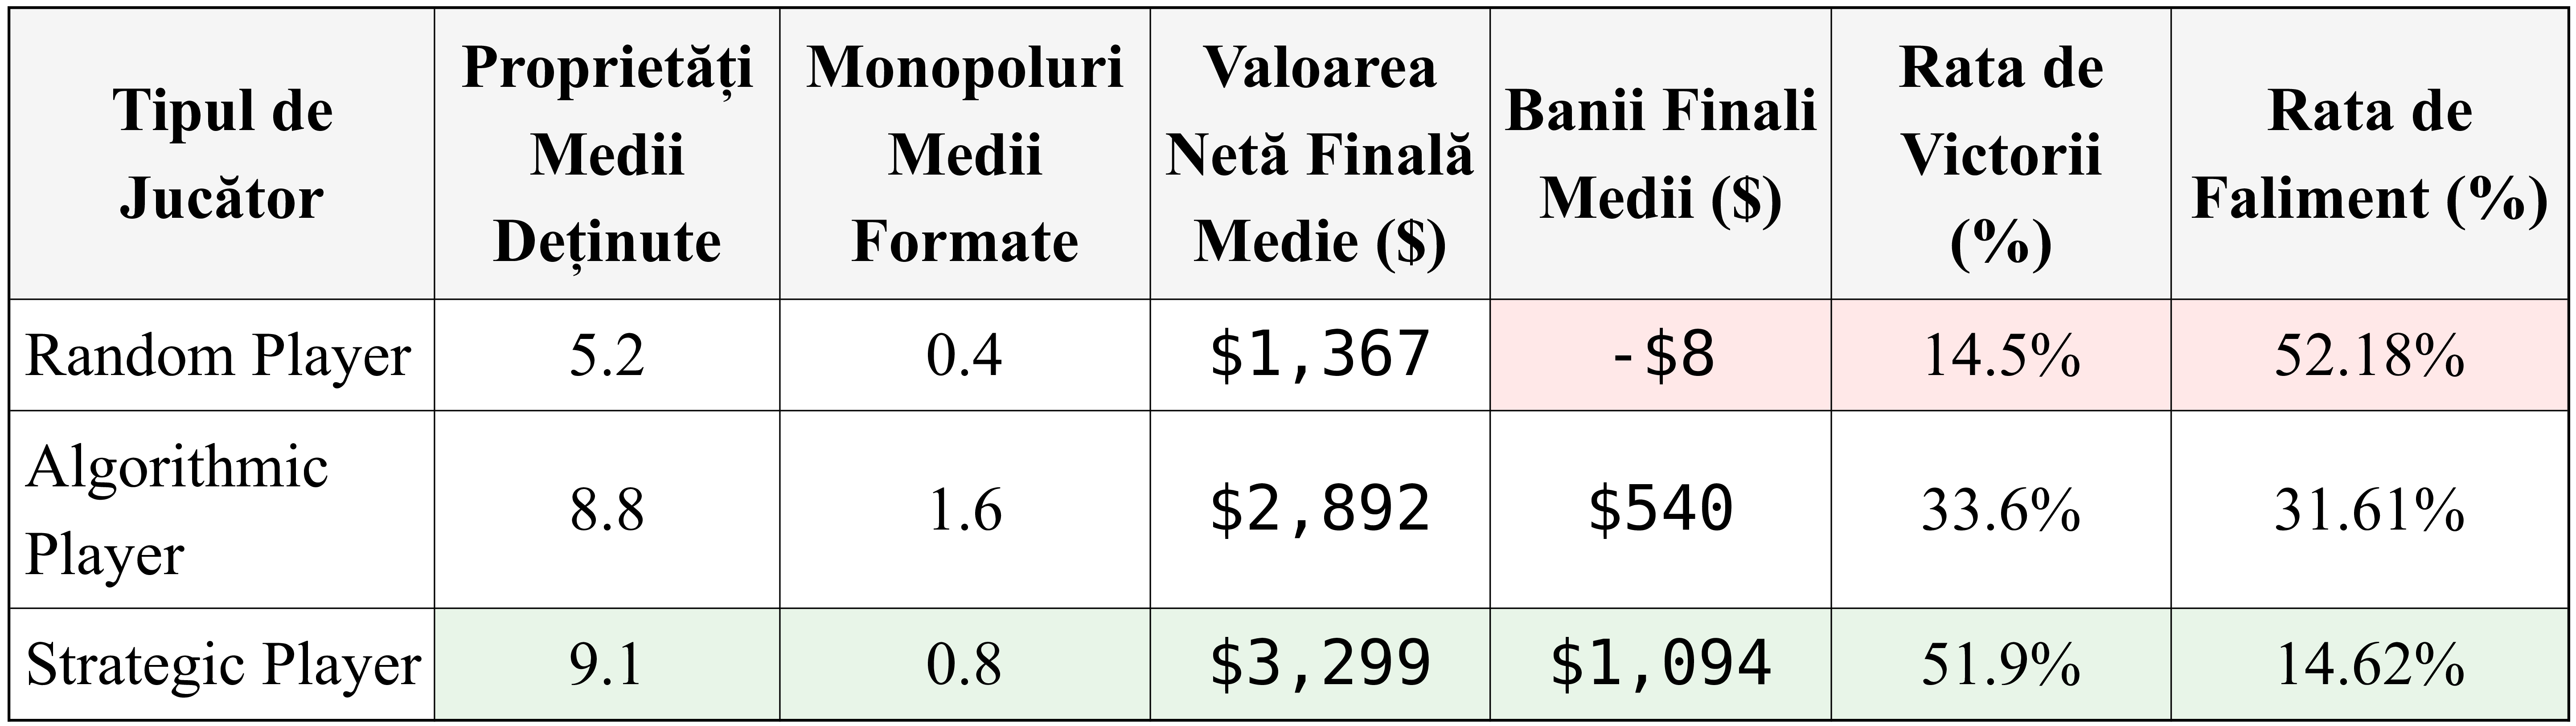
\includegraphics[width=16cm]{images/tournament_results_table.png}
    \caption{Rezultatele turneului agenților algoritmici}
    \label{fig:tournament-results-algorithmic}
\end{figure}

Suma negativă a jucătorului aleator nu este o greșeală, ci reflectă că adesea el este motivul încetării jocului, rămânând falimentar în foarte multe cazuri. Diferența dintre cei doi jucători algoritmici este una vizibilă, cel strategic preferând să aibă o rezervă cât mai mare de cash, ce îi asigură fluiditate și stabilitate.

\begin{figure}[H]
    \centering
    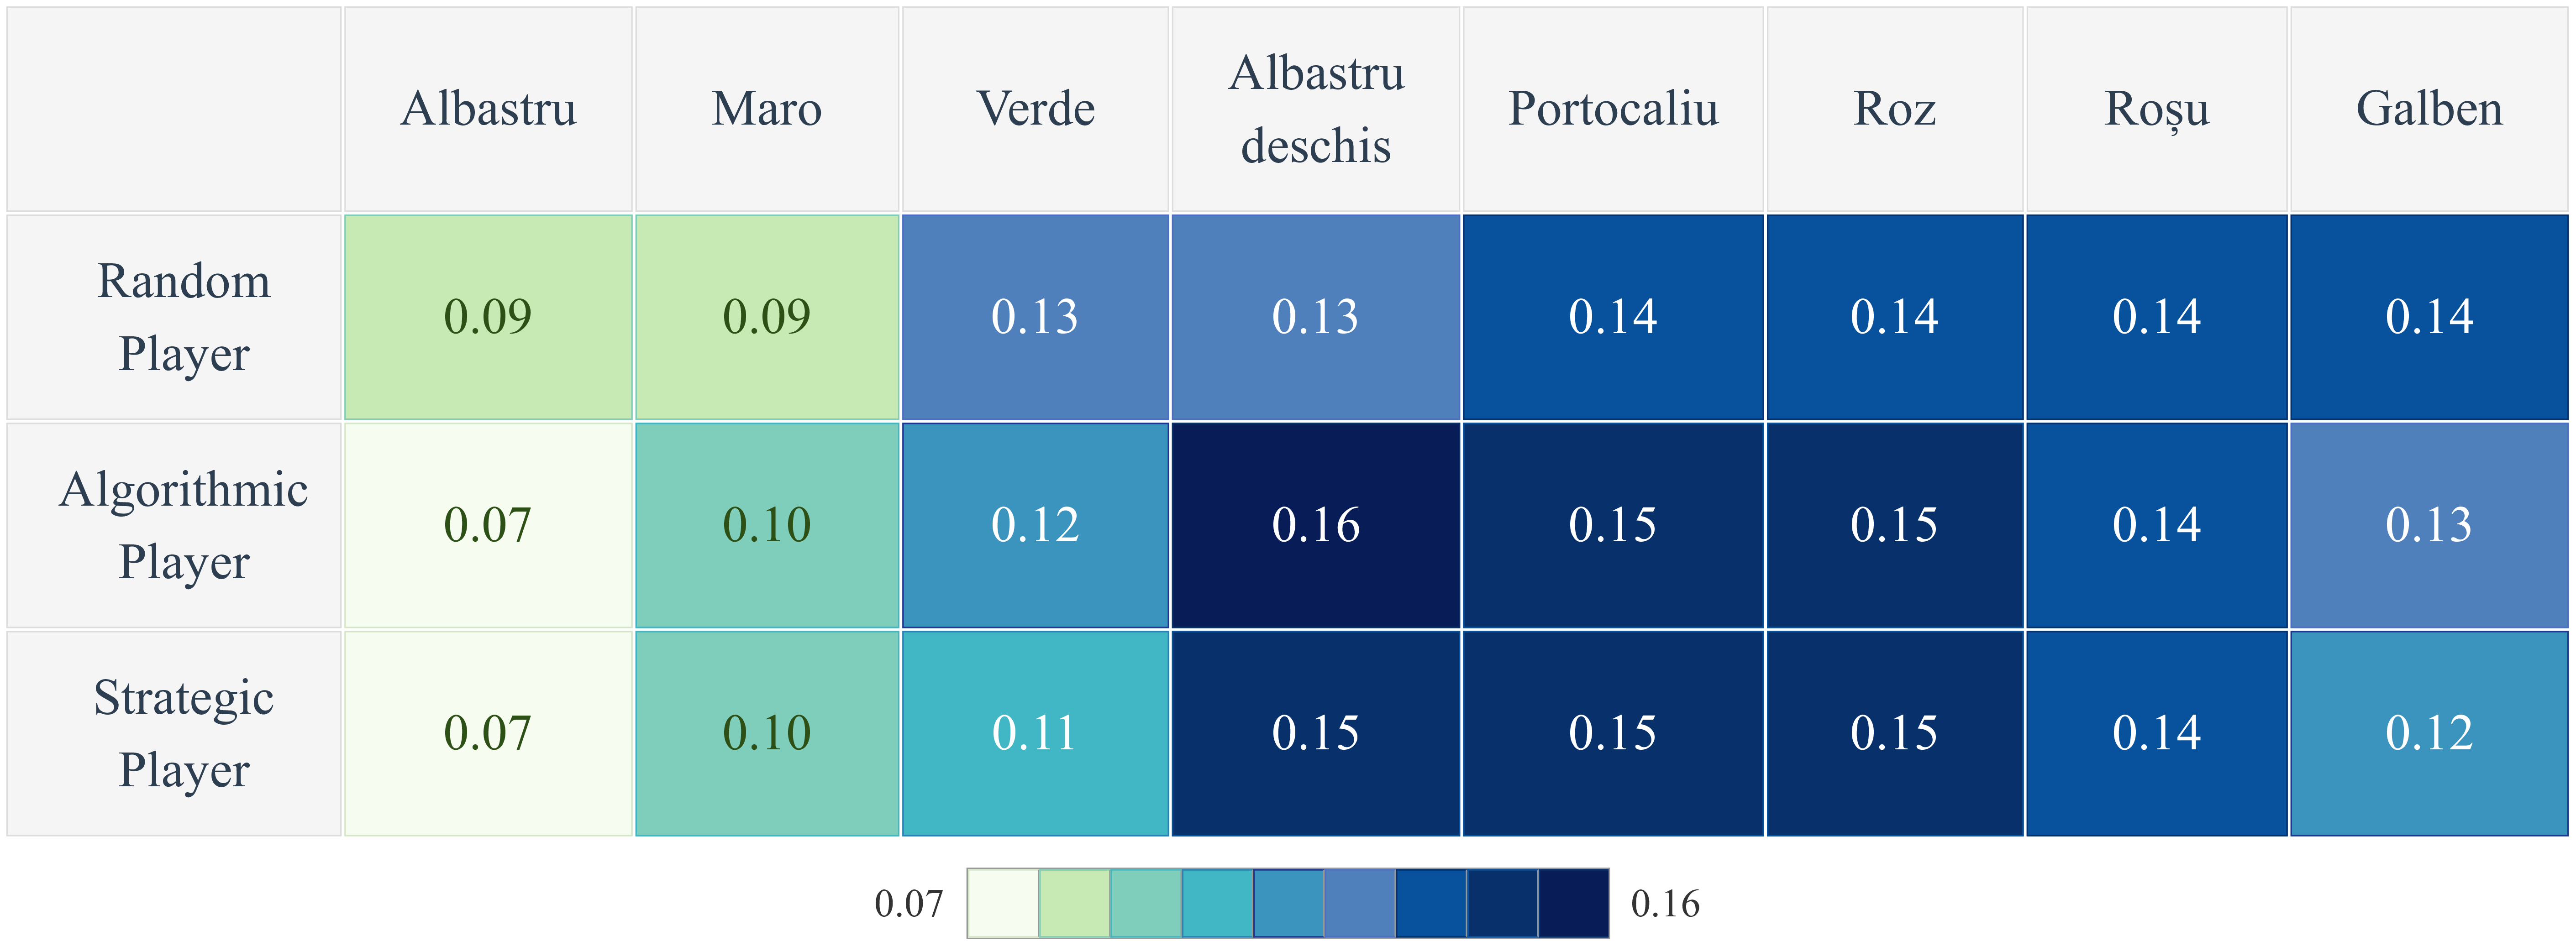
\includegraphics[width=16cm]{images/algorithmic_tournament_property_preferences.png}
    \caption{Preferințele achiziționării grupelor de culoare din turneul agenților algoritmici}
    \label{fig:tournament-results-algorithmic-property-group-preferences}
\end{figure}

În figura \ref{fig:tournament-results-algorithmic-property-group-preferences} se poate observa lipsa unei strategii definitorii în cazul agentului aleator, acesta cumpărând orice proprietate, reflectând distribuția aruncării zarurilor, frecvența fiind ridicată în jurul grupurilor de culoare vizitate regulat de jucători. Cei doi agenți algoritmici, în schimb, preferă să achiziționeze aceste proprietăți, specific grupurile de culoare albastru deschis, portocalii și roz, având o bună frecventare, dar și o bună marjă de profit.

În cazul meciurilor duel, agentul aleator a reușit să câștige în 32\% din instanțe versus agentul algoritmic și în 12\% din instanțe în fața celui strategic. Aceste numere arată, că deși deciziile sale sunt pur stocastice, acesta reușește totuși să găsească o strategie optimă. Totodată aceste numere ne indică un adevăr enunțat anterior, că o strategie universal valabilă este greu de modelat în cazul unui algoritm generalist.

Agentul strategic reușește să câștige în 67\% din instanțe față de cel algoritmic, fapt ce demonstrează că acesta este o îmbunătățire considerabilă. Diferența de 20\% în fața agentului aleator indică că strategia aleasă de agentul strategic reușește să acopere mai multe cazuri și indică o mai bună cunoaștere a mediului și a folosirii informației din acesta.

\begin{figure}[H]
    \centering
    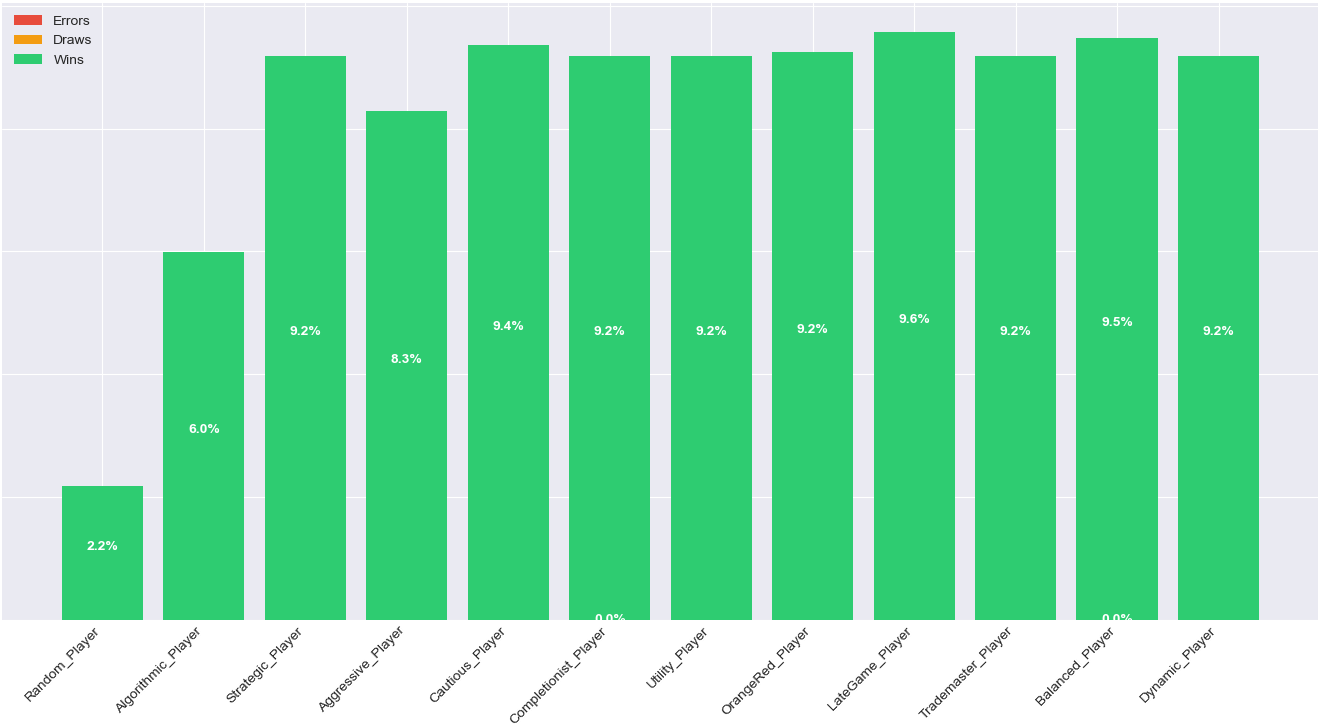
\includegraphics[width=16cm]{images/all_algorithmic agents tournament_win_rates.png}
    \caption{Rezultatele turneului round-robin pentru toți agenții algoritmici}
    \label{fig:all_algorithmic_tournament}
\end{figure}

Figura \ref{fig:all_algorithmic_tournament} prezintă rata de câștig pentru fiecare tip de agent descris până acum, într-un turneu round-robin cu 660.000 de jocuri (10.000 pentru fiecare pereche), 1.000 de runde maxime pentru fiecare joc. Așa cum se poate observa, deși are mișcări aleatoare, primul agent reușește să adune 2,2\% rată de câștig ceea ce marchează că imprevizibilitatea lui este greu de estimat de orice implementare.

La polul opus, se poate deduce că agentul strategic, cu parametrizare standard, este un jucător redutabil, având rata de câștig de 9,2\%, chiar media agenților strategici. Configurația LateGame (proiectare viitoare) este cea care reușește să se remarce cel mai bine cu o rată de câștig de 9,6\%. Atuurile acestuia sunt păstrarea unei rezerve minime de cash de cel puțin 250₩, o diferență de 100₩ față de configurația standard, și o adaptabilitate dinamică în funcție de etapele jocului, care actualizează parametrizarea agentului.

Se poate observa că media agenților strategici este 9,25\%, fiind relativ mare față de o medie a unui turneu cu agenți ce ar fi generat o rată de câștig dintr-o distribuție uniformă, 8,33\% ($100\% / 12$ (agenți)), demonstrând astfel capacitatea de adaptare și acționare într-un mediu dinamic al agenților.

\newpage
\section{Agentul uman}
În vederea interacțiunii și testării agenților, s-a realizat o interfață grafică, considerată a fi agentul uman. Aceasta are aceleași metode puse la dispoziție, iar deciziile sunt efectuate de un jucător uman.

Arhitectura agentului este una de tipul RESTful, folosind un server pe partea de backend si o interfață web pe partea de frontend. Printre tehnologiile folosite pentru realizarea interfeței grafice se enumeră: React \cite{react_dev}, Javascript \cite{mdn_javascript}, Bootstrap \cite{bootstrap}, FastAPI \cite{fastapi}, Python \cite{python_org}.

Serverul este notificat de către GameManager când un eveniment a avut loc, prin metodele legate de evenimente si păstrează cererea într-o coadă de priorități blocantă. Atunci când jocul necesită decizia jucătorului uman în privința oricărei acțiuni, se verifică existența acestei decizii în coada blocantă. În cazul în care aceasta nu există, metoda notifică interfața web despre nevoie de decizie, iar aceasta își actualizează aspectul și asteaptă pentru ca jucătorul să întreprindă o acțiune. În urma răspunsului primit de la jucator, interfața partajează acțiunea serverului, care returnează maparea la tipul cerut de metodă și încheie acțiunea curentă.

\begin{figure}[H]
    \centering
    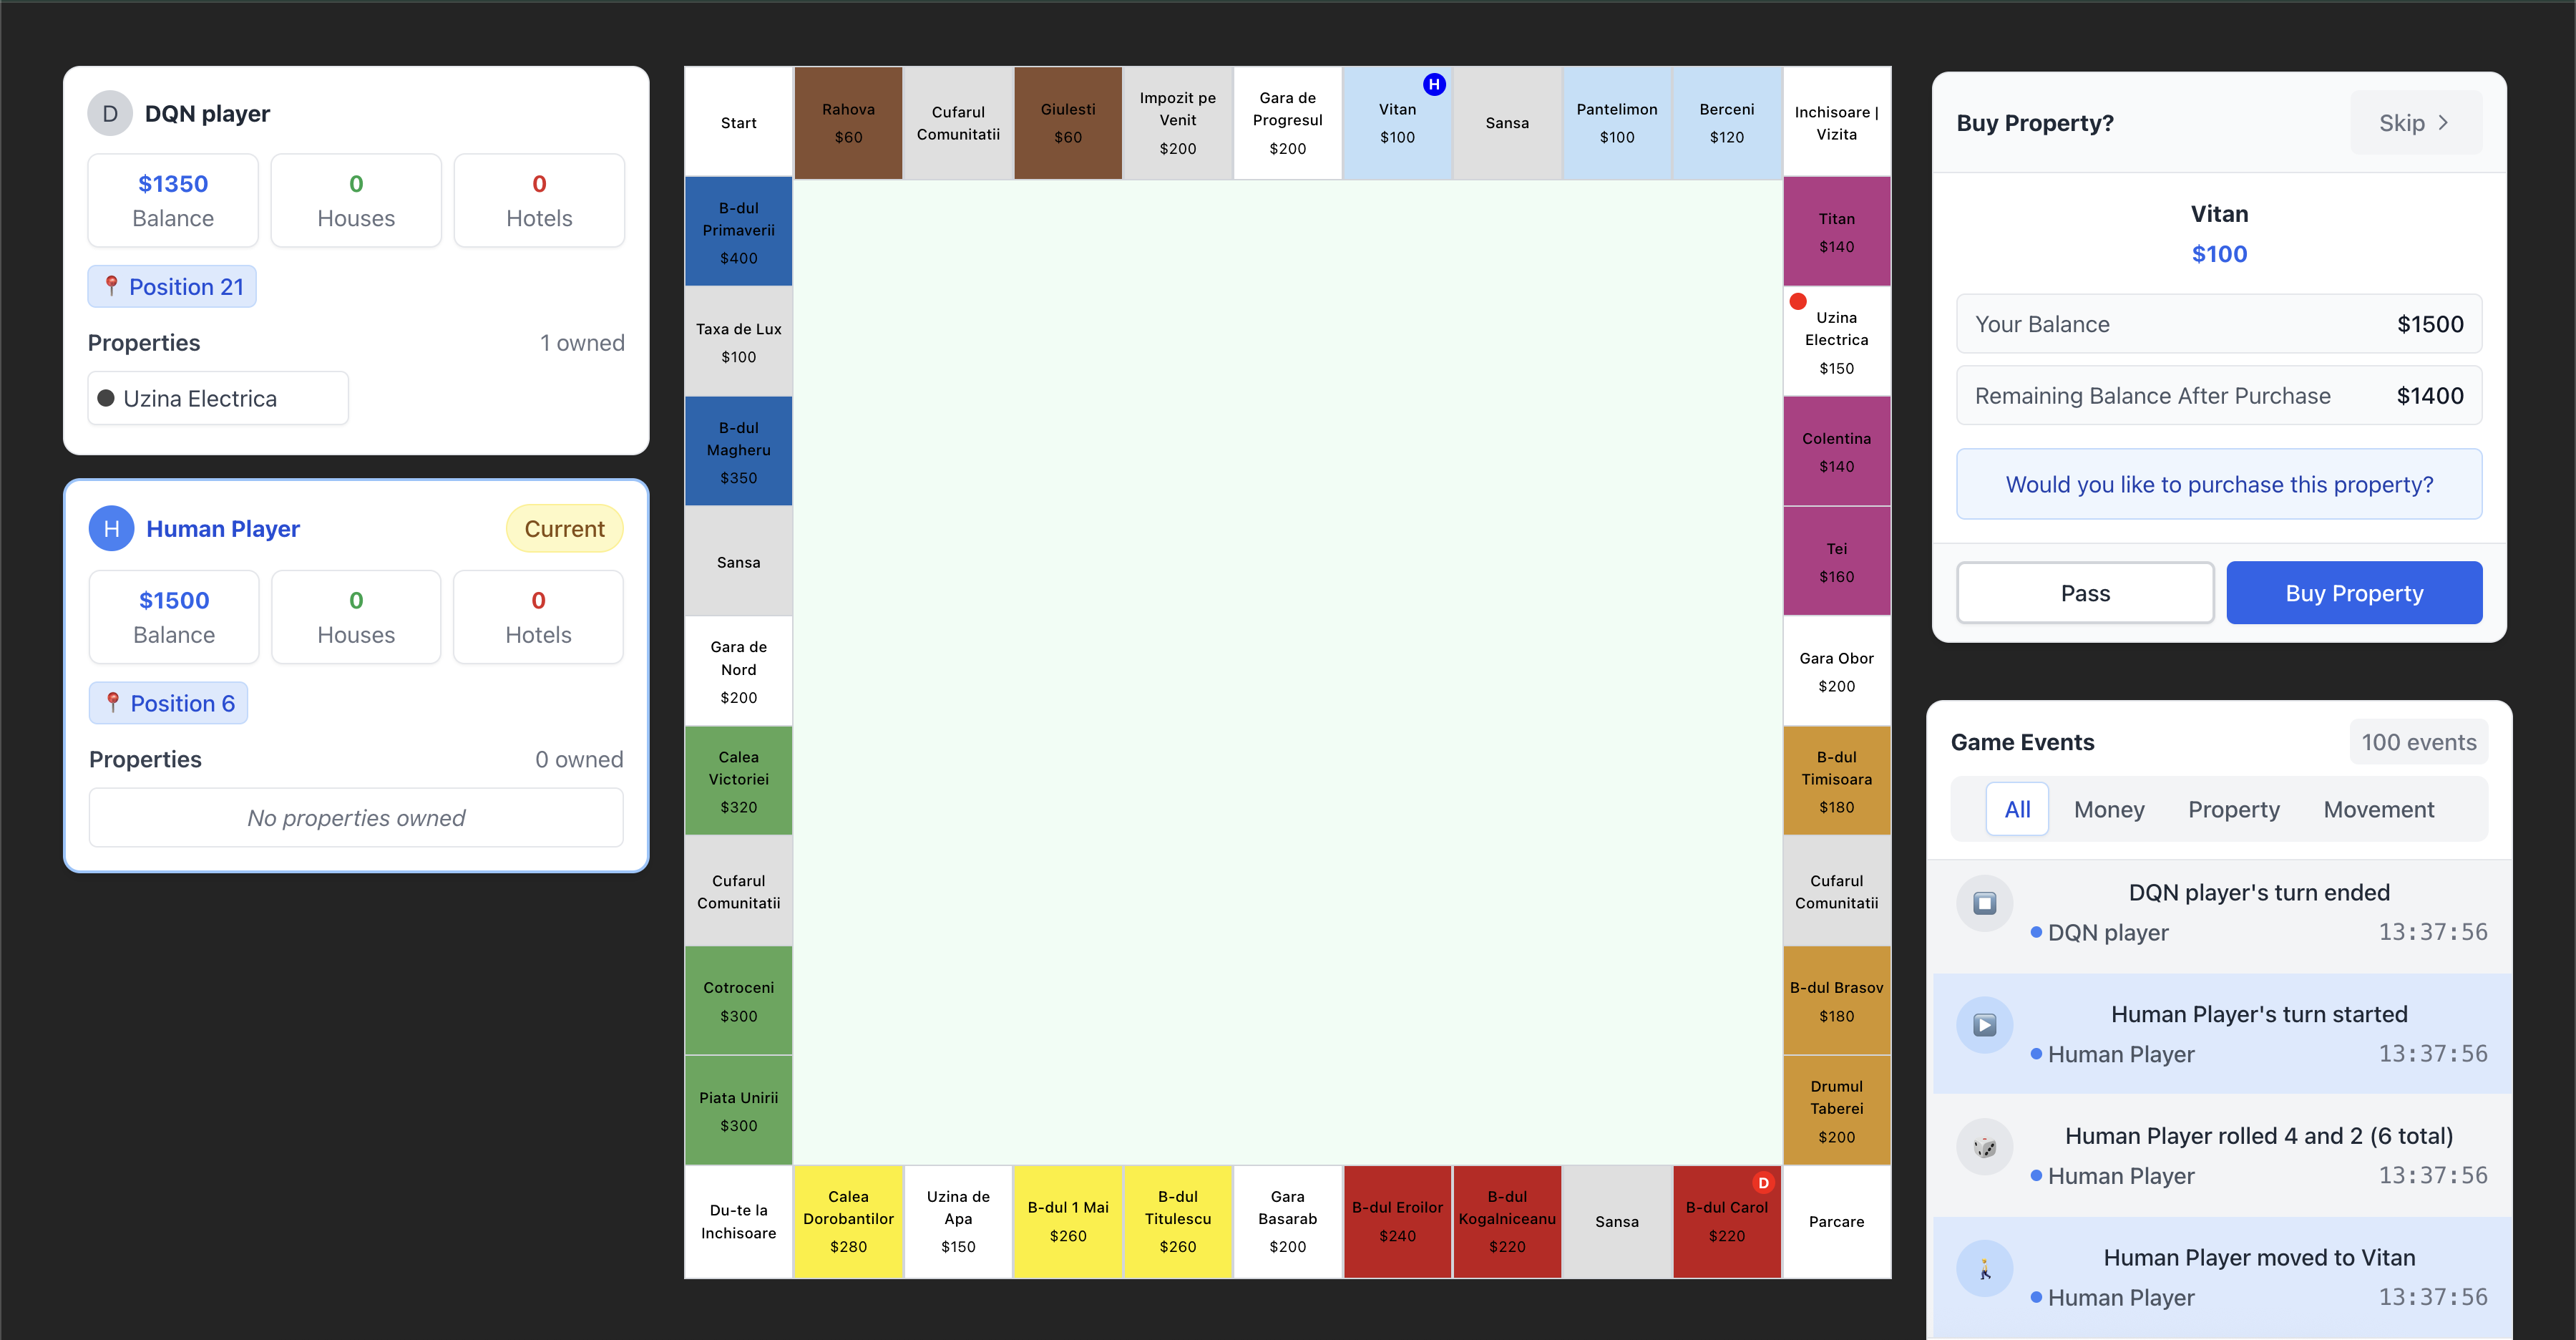
\includegraphics[width=16cm]{images/screenshot_GUI.png}
    \caption{Captură de ecran al interfeței grafice al jucătorului uman}
    \label{fig:screenshot-human-player-gui}
\end{figure}
\chapter{Agentul DQN}

\section{Contextul curent}
În ciuda popularității sale accentuate și al bazei mari de jucători, preponderent observată în ultimii ani, jocul Monopoly nu s-a bucurat de o prezență impunătoare în cazul studiilor efectuate pentru învățarea automată. Multe studii timpurii \cite{mdp_monopoly_1}, \cite{mdp_monopoly_2} și-au bazat cercetarea ca pură definire a abordării modelării jocului ca un proces Markov, iar o lucrare mai recentă \cite{mdp_monopoly_3} a concretizat efortul anterior și ca un proces decizional Markov.

O încercare de abordare hibridă a putut fi observată în cadrul lucrării \cite{hybrid_monopoly}, unde autorii s-au remarcat prin folosirea metodelor algoritmice în cadrul acțiunilor nefavorabile învățării prin întărire, precum cele care ar fi necesitat o colectare îndelungată de date, dat fiind caracterul lor sporadic, precum decizia utilizării unui cartonaș de ieșit din închisoare. Totuși, abordarea lor presupunea folosirea unei singure rețele pentru antrenarea și prezicerea acțiunilor, lucru ce poate îngreuna acuratețea și perspicacitatea deciziilor.

Cercetarea condusă a demonstrat că nicio lucrare menționată anterior sau precursoare al acestora nu a considerat o arhitectură bazată pe mai multe rețele neuronale atribuite fiecărei acțiuni. Totodată se remarcă lipsa unei abordări a unui sistem expert, menite să reducă timpul de antrenare și îmbunătățească abilitatea agentului de învățare \cite{expert_learning}. Conform programului de antrenare în vederea găsirii unei abordări dinamice pentru jocul GO \cite{alphago}, învățarea supervizată folosind o bază de date de 30 de milioane de experiențe colectate, au reușit să reducă semnificativ timpul de antrenare inițială al modelului.

\section{Arhitectura hibridă}
\subsection{Motivația pentru arhitectura hibridă}
Așa cum am văzut până acum, proiectarea unei politici optime este imprecisă și nefezabilă, din punct de vedere al timpului investit în gândirea și proiectarea algoritmului dar și a testării și evaluării sale obiective. De aceea lucrarea curentă își propune evidențierea și utilitatea unei abordări hibride în scopul obținerii unor rezultate excelente care să depășească cu un proces remarcant agenții algoritmici.

Introducerea unei astfel de decizii de design își are fundamentele pe avantajele conferite:
\begin{itemize}
    \item \textbf{Specializarea pe domenii specifice}: Ne putem focaliza pe implementarea rețelelor neuronale pentru acele metode fezabile și putem folosi implementarea algoritmică pentru celelalte metode.
    \item \textbf{Eficiența antrenamentului}: Vom putea reduce timpul necesar și complexitatea codului, având în vedere antrenamentul metodelor fezabile.
    \item \textbf{Flexibilitate arhitecturală}: Posibilitatea de a folosi sau nu a metodelor pe baza de rețele neuronale independente.
\end{itemize}

\subsection{Integrarea cu agentul strategic}
Agentul DQN este implementat ca o extensie a agentului strategic, folosind tehnica de moștenire din Python \cite{python_inheritance}, pe baza căreia, toate metodele sunt public accesibile și folosibile, având posibilitatea de a decide modul de operare curent al fiecărei acțiuni, așadar putând decide modul de tranziționare graduală de la algoritmii clasici la învățarea automată.

Abordarea moștenirii oferă posibilitatea de asigurare a tratării excepțiilor prin întreprinderea metodelor părinte, fapt ce asigură un comportament complet funcțional. De asemenea integrarea și adăugarea ulterioară a metodelor se poate face treptat, fără a avea nevoie de o structură monolitică a compunerii agentului, folosind metodele deja expuse, ulterior înlocuindu-le o versiune îmbunătățită. Testarea metodelor devine și ea trivială, fiind facilitatea de izolare a metodei folosite și observarea procentului de implicare în rata de câștig.

\subsection{Separarea deciziilor}
Deși o componentă importantă, ce reușește să rezolve și îmbunătățească numeroase conflicte de interes, schimbul rămâne o acțiune incertă și doar un refugiu în privința incrementării averii din joc. Datorită complexității ridicate de encodare a unei oferte de schimb, a proiectării unei funcții optime de recompensă și a frecvenței reduse de observații, metodele aferente schimbului au fost complet excluse din faza învățării automate și tratate prin folosirea metodelor părinte.

De asemenea, tratarea metodei de recuperare din faliment a fost preluată din părinte, aceasta având o rată mică de apariție în joc, dar și datorită numeroaselor aspecte implicate, precum decizia de ierarhizare a pașilor în rezolvarea falimentului, prioritizare obiectivelor de scurtă durată și influența rezolvării conflictelor financiare.

Celelalte metode prezentate în tabelul \ref{fig:player_interface_methods} vor fi implementate folosind paradigme învățării automate, prin rețele neuronale de tipul Q (Deep Q-Networks, DQN). În urma testelor efectuate, s-a realizat că pentru anumite metode de modificare a posesiunilor, rețelele nu reușeau să surprindă eficient pericolele viitoare ale deciziilor curente, precum ipotecarea sau vânzarea caselor/hotelurilor. Așadar s-a considerat utilizarea unei abordări mixte, prin executarea acțiunii rețelei, doar când metoda părinte ar fi considerat benefică efectuarea acțiunii. Astfel, s-a observat o creștere de 33\% comparativ cu o abordare statică ce considera doar rezultatul rețelei.

Considerentele ce ar putea fi implicate sunt greu de concretizat, dar presupunerea proprie observată în urma experimentelor arată că rețeaua nu a reușit să capteze în totalitate consecințele viitoare ale unei acțiuni distructive.

\section{Rețele de tipul Q}
Într-un mediu cu număr de stări și acțiuni predefinit, relativ mic, se pot folosi matrici bidimensionale pentru maparea valorilor Q pentru fiecare pereche de stare și acțiuni, astfel construindu-se o reprezentare detaliată a politicii optime. Din păcate, într-un mediu dificil de reprezentat și configurat, cu un număr impunător de tranziții de stări și acțiuni, această mapare ar fi imposibil de realizat datorită dimensiunilor reduse ale memoriei, dar și din cauza timpului îndelungat necesar explorării tuturor tranzițiilor pentru generarea unei politici optime. Ca și referință putem avea în vedere un joc de șah, în care s-a estimat că totalitatea stărilor posibile ar fi aproximativ $10^{43}$ \cite{shannon1950chess}, un număr extraordinar, comparativ cu puterea de calcul și stocare actuală.

Astfel, rețelele neuronale sunt folosite pentru replicarea mapării, generând o funcție de mapare, în loc să păstreze valorile mapate. Acest lucru simplifică spațiul de stocare necesar, fiind o alternativă viabilă în cadrul spațiilor vaste de acțiune. Acestea au ca argument (input) reprezentarea vectorială a stării curente (embedding) și oferă aproximarea valorii Q ca și rezultat (output).

\subsection{Encodarea stării. Spațiul de acțiuni}\label{state-embeding}
În vederea realizării encodării stării, s-a plecat de la datele avute la dispoziție și expuse de reprezentarea oferită de GameState. Astfel s-a decis încorporarea lor într-o formă vectorială, într-un spațiu real cu 100 de dimensiuni. Reprezentarea dimensională a fost făcută doar pentru regulile predefinite, plecând cu presupunerea că vor exista doar doi jucători pe parcursul oricărui joc. Aceasta s-a făcut într-o formă alternativă, plecând cu informația agentului curent, urmată de informația oponentului, secvențial pentru fiecare categorie, după cum urmează:
\begin{itemize}
    \item \textbf{Informațiile jucătorilor (8 caracteristici)}: pozițiile pe tablă, balanțul cash, statutul libertății, cărțile de ieșire din închisoare.
    \item \textbf{Indicatori al monopolurilor (48 de caracteristici)}: deținerea proprietăților, al caselor/hotelurilor, al proprietăților ipotecate.
    \item \textbf{Contextualizare strategică (44 de caracteristici)}: gradul de progres al jocului, gradul de apreciere al utilităților, numărul turelor în închisoare, etc.
\end{itemize}

\begin{figure}[H]
    \centering
    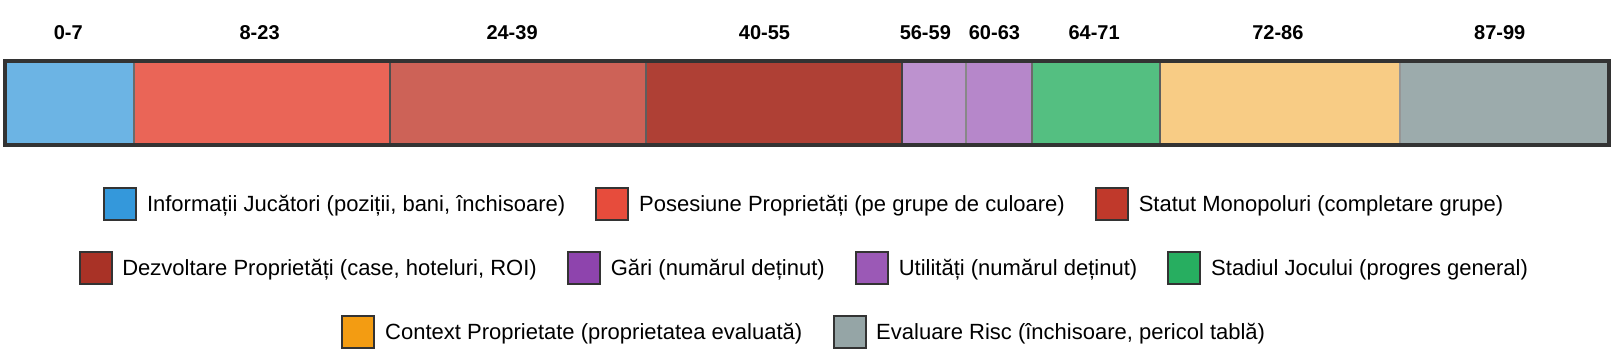
\includegraphics[width=16cm]{images/vector_visualizer.png}
    \caption{Vizualizarea distribuției informației în encodarea stării}
    \label{fig:state-distribution}
\end{figure}

Conform observațiilor recente \cite{drl_normalization_benefits}, normalizarea datelor în procesul de preprocesare aduce multiple beneficii precum reducerea pierderilor datorate unei înclinații (bias) nefavorabile în mediu, cât și asigurarea unei convergențe mai bune în scopul obținerii unei politici optime.

Rezultatele observate folosind normalizarea datelor în procesul de embedding, au fost comparate cu o abordare nenormalizată, observându-se atât un rezultat superior în cazul ratei de câștig, cât și o politică mai bună în cazul testelor cu un agent uman.

Limitele folosite în marginire au fost fie evidente, precum numărul maxim de cărți de ieșit din închisoare (2), număr predefinit de regulile jocului, fie alese în urma rulării mai multor mii de jocuri și colectării de date, având o marjă de incrementare considerabilă (aproximativ 30\%) cu scopul evitării și minimizării utilizării de valori supraunitare. De exemplu balanța cash a fiecărui jucător a fost raționalizată în funcție de o sumă maximă de 5.000₩.

Asemănător acțiunilor prezentate în tabelul \ref{fig:player_interface_methods}, dimensionalitatea metodelor a fost păstrată integral, excepție făcând metodele de ipotecare și dezipotecare, care au avut în cazul implementării dimensiunea de 40, corespunzătoare fiecărei căsuțe de pe tablă. Aceasta s-a realizat în urma observării unui rezultat net inferior păstrării numărului de 22 de celule aferent tuturor proprietăților cumpărabile. Ipoteza emisă este greu de justificat, dar este probabil ca rețeaua să prefere o discretizare apropiată de factorul de normalizare folosit anterior pentru raționalizarea căsuțelor și a pozițiilor.

\section{Designul rețelelor neuronale}
\subsection{Rețele multiple}
O contribuție majoră a acestei implementări a fost folosirea multiplelor rețele neuronale pentru fiecare tip de decizie. În lucrările anterioare (\cite{mdp_monopoly_2}, \cite{hybrid_monopoly}), autorii au abordat problema utilizând o singură rețea neuronală cu ieșire fie binară, fie terțiară, utilizând diferite abordări cu scopul utilizării sale în acțiuni cu o dimensionalitate diferită, precum cea a îmbunătățirii unei proprietăți.

Această abordare avea avantajul simplificării atât a procesului de învățare, cât și a evaluării politicii obținute. Totuși, conversia dintre spațiile dimensionale diferite se făcea urmând o abordare algoritmică ceea ce ducea la o lipsă directă de înțelegere a consecințelor și reprezentării fidele ale acțiunii.

Așadar, curenta lucrare și-a propus definirea câte unei rețele proprii pentru fiecare acțiune, ce urmează să fie antrenată independent față de celelalte, mapând corect ieșirile la dimensionalitatea cerută de fiecare acțiune. Prin aceasta se urmărește obținerea unei scalabilități crescute și o convergență ridicată ce se focalizează pe izolarea principiilor decizionale și a concretizării spațiului fiecărei acțiuni.

Pentru implementare s-a folosit librăria (framework-ul) Tensorflow \cite{tensorflow}, unul dintre cele mai răspândite în cazul domeniului inteligenței artificiale. Acesta a fost prioritizat datorită implementărilor simpliste și eficiente, favorizând scrierea de coduri rapid și oferind suport pentru multiple platforme.

\subsection{Arhitectura rețelelor. Hiperparametrii}
Fiecare rețea posedă o structură comună ce este menită să ușureze implementarea și ofere posibilitatea de scalare rapidă. Aceasta constă dintr-un strat (layer) linear \cite{tensorflow_linear} de intrare (input) de dimensiuni 100, pentru acoperirea tuturor parametrilor descriși în encodarea stării \ref{state-embeding}. Acesta este continuat de o secvență de 3 straturi liniare cu dimensiunile 128, 64, 32, respectiv, urmat de stratul linear de ieșire cu dimensiune variabilă, în funcție de metoda adaptată. Între straturi, cu excepția ultimului, se aplică o funcție de activare liniară (rectified linear unit, ReLU \cite{tensorflow_relu}), menită să spargă liniaritatea, oferind posibilitatea de învățare a trăsăturilor non-liniare.

Pentru configurația hiperparametrilor s-au ales următoarele valori:
\\
\[
\begin{array}{ll}
\text{Rata de învățare } \alpha & 0.001 \text{ (Optimizator Adam)} \\
\text{Factorul de discount } \gamma & 0.99 \\
\text{Epsilon inițial } \epsilon_{\text{start}} & 1.0 \\
\text{Epsilon final } \epsilon_{\text{end}} & 0.1 \\
\text{Rata de decrementare } \gamma_\epsilon & 0.995 \\
\text{Rata de actualizare a rețelei scop (target network) } \tau & 10 \\
\text{Batch size} & 64
\end{array}
\]

\section{Procesul de antrenare}
În vederea antrenării metodelor ce utilizează rețele neuronale s-a propus antrenarea pe rând a fiecărei metode, urmând o ordine specifică, prioritizarea acestora făcându-se pe baza importanței și frecvenței folosirii în joc. Metoda supusă antrenării, va urma două faze distincte: \textbf{antrenarea cu un expert} și \textbf{antrenamentul prin experiențe proprii}.

Din datele colectate, pe baza a milioane de simulări, s-a constatat că metoda de cea mai mare importanță, având totodată și o frecvență ridicată de folosire, este cea de decidabilitate a achiziționării unei proprietăți. Această observație este una destul de intuitivă, având în vedere că în lipsa proprietăților majoritatea acțiunilor din joc își pierd scopul. Urmată de aceasta, metodele de îmbunătățire și renunțare la case/hoteluri, au fost cele care au fost observate imediat, acestea facilitând producerea de venituri, demonstrează că o maximizare a încasărilor este ceea ce conduce la un câștig sigur. Și nu în ultimul rând, deciziile distructive, precum cea de ipotecare și dezipotecare au fost observate ca având o influență relativ scăzută, probabil datorită caracterului lor ambiguu, folosirea acestor metode realizându-se doar în cazuri extreme de posibilă lichidare, altminteri, utilizarea lor putând reduce dramatic șansa de câștig. Deciziile corelate cu închisoarea, au fost din păcate, lăsate la final, datorită lipsei de frecvență în joc. Posesia unui cartonaș de ieșire din închisoare este destul de rară, fiind în joc doar două, și fiind nevoie de o deplasare până la o căsuță de șansă/cufărul comunității, iar apoi existând șansa nevoii de extragere a 15 cartonașe, până la primirea unui cartonaș căutat.

\subsection{Procesul de actualizare al ponderilor}
În cadrul oricărei rețele neuronale, vom avea nevoie de definirea unei funcții de pierdere (loss function) care ne va ajuta să actualizăm parametrii rețelei, indicând direcția corectă de deplasare și valoarea gradientului, astfel încât predicțiile noastre să se îndrepte către un punct de minim local dorit.

Abordarea DQN presupune actualizarea valorii Q pe baza diferenței temporale dintre valorile estimate, a recompensei obținute, ponderate de rata curentă de învățare, așa cum se poate vedea în ecuația \ref{eq:dqn-update-rule}.

\begin{equation}\label{eq:dqn-update-rule}
    Q(s_t, a_t) \leftarrow Q(s_t, a_t) + \alpha(R_{t+1} + \gamma \max_a Q(s_{t+1}, a) - Q(s_t, a_t))
\end{equation}

Pentru stabilitatea învățării s-a utilizat o rețea scop (target network), ce are ca rol predicția stării așteptate, pentru evitarea ciclurilor de feedback și apariția problemei estimării celor două valori Q într-un interval scurt \cite{milvus_target_networks}. În absența acesteia, rețeaua curentă ar fi fost responsabilă pentru aproximarea valorii Q așteptate, fapt ce ar fi condus la actualizarea acesteia după fiecare pas, făcând procesul de antrenare instabil.

De asemenea, pentru concretizarea unui proces sigur și stabil de învățare, s-a construit o zonă de memorie pentru redarea experiențelor (replay buffer) ce asigură actualizarea graduală a ponderilor rețelei, pentru evitarea instabilităților numerice \cite{lazyprogrammer_replay_buffer}. Importanța acesteia este reliefată de amortizarea impactului fiecărei experiențe participante la procesul de îmbunătățire a rețelei. Fără aceasta, procesul de actualizare s-ar fi făcut pe experiențe consecutive, fapt ce ar fi condus la posibilitatea unui factor de bias temporal. Prin amestecarea experiențelor și extragerea acestora grupate, se ameliorează rata de actualizare în scopul evitării unei reduceri sau îmbunătățiri drastice.

\begin{equation}\label{eq:loss-funciton}
    \mathcal{L}(\theta) = \frac{1}{|\mathcal{B}|} \sum_{i \in \mathcal{B}} \text{Huber}_\delta(y_i - Q_\theta(s_i, a_i))
\end{equation}

Definim astfel funcția de pierdere în ecuația \ref{eq:loss-funciton}, unde $y_i$ reprezintă valoarea Q calculată cu rețeaua scop. Această funcție măsoară diferența dintre predicțiile rețelei și valorile așteptate, ghidând procesul de optimizare către soluția optimă. Utilizarea funcției Huber asigură stabilitate numerică pentru erorile mici și robustețe pentru valorile extreme, facilitând convergența în condiții variate de antrenament.

\begin{equation}\label{eq:update-rule}
    \theta \leftarrow \theta - \alpha_{\text{Adam}} \nabla_\theta \mathcal{L}(\theta)
\end{equation}

Actualizarea parametrilor rețelei principale se va face după fiecare episod prin ecuația \ref{eq:update-rule}, iar cea a rețelei scop la fiecare 10 episoade, pentru prevenirea instabilităților descrise anterior.

\subsection{Învățarea expert}
Pentru fiecare metodă antrenată s-a considerat ca și etapă inițială, folosirea experiențelor preluate din redarea jocurilor unor agenți experți, configurația de bază a agentului strategic, LateGameDeveloper și CautiousAccumulator, cele mai bune 3 configurații obținute în urma rulării multiplelor turneuri.

Experiențele au fost colectate într-un număr total variabil (50 de milioane de experiențe pentru metoda de achiziționare a unei proprietăți, 70 de milioane pentru cea de îmbunătățire, etc.), iar apoi folosite pentru actualizarea ponderilor descrisă în secțiunea anterioară.

Prin aceasta s-a urmărit stimularea înțelegerii jocului Monopoly, dar mai important, însușirea regulilor de bază. În ciuda simplității lor, regulile jocului Monopoly, sunt greu de generalizat și însuțit într-o formă matematică. De aceea, prin învățarea supervizată a unui expert, agentul a reușit să acumuleze într-un timp record regulile acestea și să poată evita situațiile de producere a unei erori.

\subsection{Antrenamentul prin experiența proprie}
După faza de antrenare supervizată, agentul a fost lăsat să învețe și descopere noi strategii prin participarea activă în jocuri de Monopoly. Inițial acesta a fost preocupat de explorarea cât mai mare a strategiilor, urmând ca apoi pentru restul 25\% din jocurile totale să urmeze o politică agresivă de exploatare cu scopul determinării strategiei optime.

La fel ca mai sus, numărul jocurilor și a timpului necesar antrenamentului a variat, în funcție de frecvența utilizării acelei metode. Astfel, pentru decidabilitatea cumpărării unei proprietăți, agentul a avut nevoie, în medie, de 20.000 de jocuri de antrenare, iar în cazul deciziei utilizării cardului de ieșire din închisoare de 50.000 de jocuri.
\chapter{Rezultate și concluzii}
\section{Evaluarea performanței}
În cadrul evaluării agentului DQN, s-a avut în vedere surprinderea ratei de câștig, a strategiei de cumpărare a proprietăților, rata de faliment, economiile și alți indicatori captați de TournamentManager.

În continuare vom presupune că toate rezultatele au fost obținute în cadrul unui turneu round-robin cu 300 de jocuri per duel, cu 1.000 de runde maxime.

\begin{figure}[H]
    \centering
    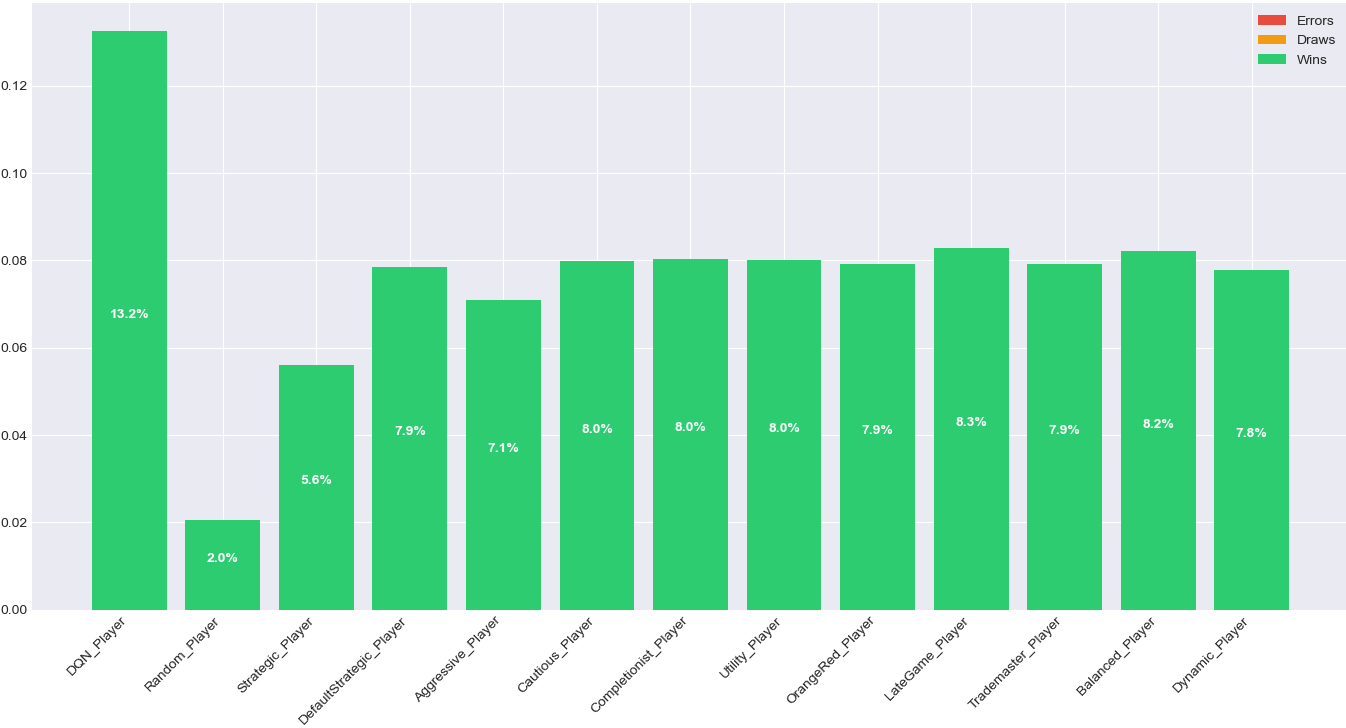
\includegraphics[width=16cm]{images/dqn_tournament_win_rates.png}
    \caption{Rezultatele agentului DQN într-un turneu}
    \label{fig:dqn-tournament-results}
\end{figure}

În figura \ref{fig:dqn-tournament-results}, se poate remarca o prezență dominantă a agentului DQN, acesta reușind să adune o rată de câștig de 13,2\%, cu 5,3\% mai mult față de agentul strategic, demonstrând adaptabilitatea și puterea acestuia de înțelegere a jocului.

Acesta a reușit să aibă o rată de faliment de doar 2\%, media fiind de 6\%, iar în cazul fluidității cash-ului acesta a reușit să adune o avere medie finală de 2321₩, de aproximativ două ori și jumătate mai mult decât media și un cash final mediu de 1865₩, de 4,1 ori mai mult decât media.

În cazul predispoziției de cumpărare, agentul DQN a preferat proprietățile din grupul verde în 30\% din cazuri, urmate de cele galbene (22\%) și albastru închis (18\%), lucru ieșit din comun, având în vedere probabilitatea statistică și rata de retur mediu al investiției. Aceasta se poate datora probabilității mari de câștig, odată securizată latura dintre căsuțele "Du-te la închisoare" și "Start", având cea mai mare chirie percepută în joc, poate lua orice jucător prin surprindere falimentându-l pe neașteptate. Astfel se poate explica și prezența mare a banilor cash la sfârșitul jocului, amintită anterior, jucătorii ajungeau pe aceste căsuțe și nu aveau resursele necesare achitării datoriilor.

Agentul DQN pare să își fi însuțit și un comportament inteligent în privința ipotecării proprietăților în vederea îmbunătățirii proprietăților. Acesta preferă să ipotecheze proprietăți pentru o scurtă durată, în vederea cumpărării caselor, când apreciază că oponentul va ajunge pe proprietățile sale. Ulterior plătirii chiriei, acesta își dezipotechează proprietățile, recuperându-și investiția.

Utilizarea abordării hibride în cazul metodelor distructive, crește rata victoriei cu 3,5\%, în cazul utilizării acesteia pentru toate metodele distructive, fapt ce semnalează prezența unei lipse de antrenare și lipsa înțelegerii depline a consecințelor viitoare.

\begin{figure}[H]
    \centering
    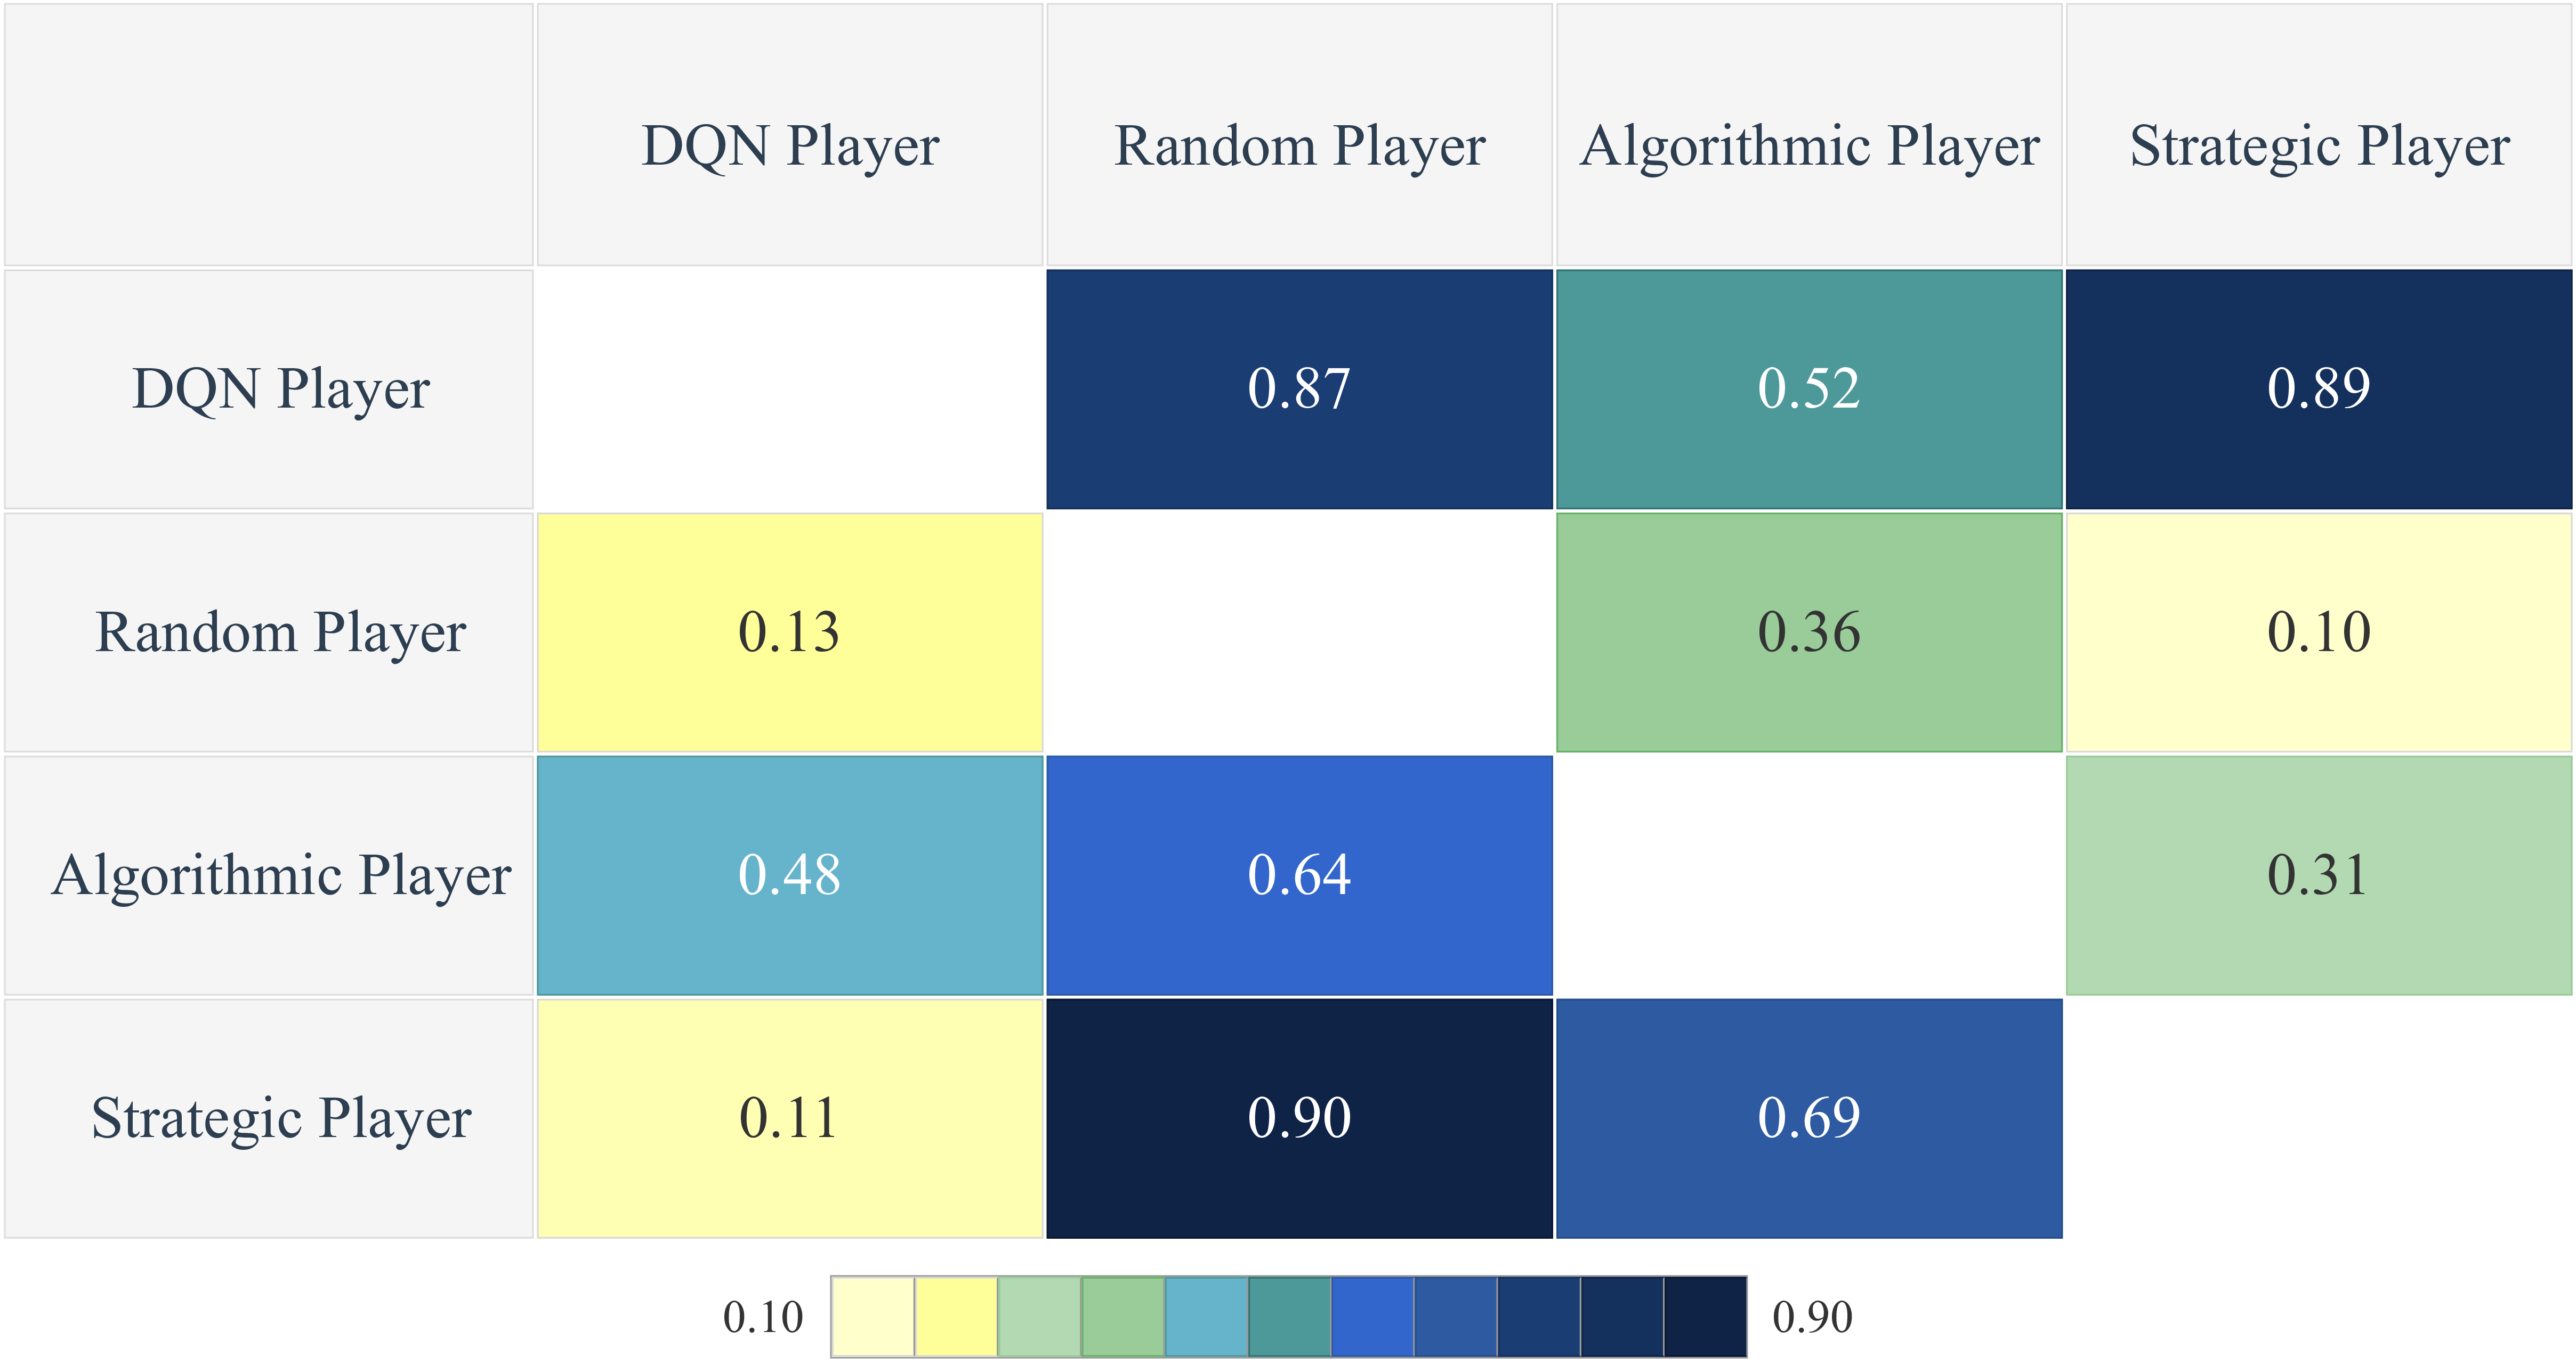
\includegraphics[width=13cm]{images/mini-tournament-dqn.png}
    \caption{Rezultatul turneului cu număr restrâns de agenți}
    \label{fig:mini-tournament-results}
\end{figure}

În cazul duelurilor cu agenții de bază, rezultatul fiind ilustrat în figura \ref{fig:mini-tournament-results}, agentul DQN pare să aibă probleme în înfrângerea celui algoritmic. O ipoteză în această privință poate consta în evitarea antrenamentelor împotriva sa, agentul algoritmic fiind folosit ca punct de "testare". Astfel, cum agentul DQN nu a fost antrenat împotriva sa, agentul algoritmic pare să introducă o strategie în fața căreia agentul DQN se poate adapta, dat fiind rezultatul de 51\% rată de câștig, dar pe care nu o poate înfrânge, dată fiind necunoscuta politică abordată.

Datorită introducerii unui eveniment neașteptat, putem oferi încă o concluzie folositoare, aceea că agentul nostru reușește să fie și robust. Într-adevăr în cazul lucrărilor amintite anterior \cite{mdp_monopoly_2}, \cite{hybrid_monopoly}, antrenamentul și testarea s-a realizat exclusiv pe baza acelorași agenți, astfel introducând un element de bias în structura decizională a agentului. Prin excluderea agentului algoritmic, am reușit să creăm o referință importantă în evaluarea sa, punct ce ne va ajuta să înțelegem cu adevărat puterea de adaptabilitate a agentului, în contextul dat, fiind una medie, reușind să depășească marja de egalitate.

\section{Dezvoltări ulterioare}
Alegerea algoritmului DQN pentru arhitectura agentului a fost inspirată din simplitatea și ușurința de implementare a acestuia, fiind baza în cadrul învățării adânci prin întărire. Deși minimalistă, această abordare poate fi mai slabă în contextul jocurilor complexe, preferându-se o variantă care învață o politică, în schimbul învățării valorilor Q.

Lucrarea \cite{hybrid_monopoly} folosește o optimizare proximală a politicii (Proximal Policy Optimization, PPO), care rezultă într-o rată de câștig comparativ mai mare față de o abordare a estimării valorii Q. Ca posibilitate de dezvoltare ulterioară aș încerca integrarea algoritmului A2C (Advantage Actor Critic), pentru observarea schimbării performanțelor și al politicii deprinse.

Aș încerca, de asemenea, modelarea și încorporarea funcției de schimb printr-un mecanism neuronal, astfel putând observa direct efectul acestora în parcursul jocului. Integrarea algoritmică nu favorizează o politică activă de schimb, ci doar o prezență pasivă în cadrul jocului, pentru a satisface nevoia de aprobare a unor schimburi existente.

\section{Aprecieri personale}
Consider că rezultatele obținute sunt satisfăcătoare și vor reprezenta un punct de plecare în considerentele viitoare. Abordarea descrisă este menită să încurajeze dezvoltări ulterioare și testări noi de teorii, oferind un sistem funcțional și scalabil.

Scopul lucrării a fost de actualizare a rezultatelor și concluzionare a unor lucrări existente, prin prisma dezvoltării unei noi abordări ușor de înțeles și de folosit.

\begin{appendix}
\chapter{Funcții de Recompensă pentru Agentul DQN}
\label{annex:reward_functions}

Această anexă prezintă formularea matematică a funcțiilor de recompensă utilizate în antrenarea agentului DQN.

\subparagraph{Recompensa de bază} Toate funcțiile de recompensă pornesc de la schimbarea normalizată a averii nete:
\begin{equation}
\Delta W_{norm} = \text{clip}\left(\frac{W_{t+1} - W_t}{200}, -1, 1\right)
\end{equation}
unde $W_t$ este averea la momentul $t$

\subparagraph{Cumpărarea proprietăților} Include bonus pentru completarea monopolurilor:
\begin{equation}
R_{buy} = \Delta W_{norm} + 0.3 \cdot I_{monopol}
\end{equation}
unde $I_{monopol} = 1$ dacă s-a completat un monopol nou, altfel 0.

\subparagraph{Îmbunătățirea proprietăților.} Combină progresul cu gestionarea lichidității:
\begin{equation}
R_{upgrade} = 1.5 \cdot \Delta W_{norm} + 0.15 \cdot \Delta H + 0.3 \cdot \Delta O + R_{lichiditate}
\end{equation}
unde $\Delta H$, $\Delta O$ sunt schimbările în case și hoteluri, iar $R_{lichiditate} = -0.2$ dacă raportul de lichiditate $L_t = C_t/W_t < 0.1$, cu $C_t$ fiind balanța de cash la momentul $t$.

\subparagraph{Vânzarea caselor/hotelurilor} Pune accent pe gestionarea cash-ului de urgență:
\begin{equation}
R_{downgrade} = 0.8 \cdot \Delta W_{norm} + R_{emergency} + R_{cash} - \sum_{g} \alpha_g
\end{equation}
unde $R_{emergency} \in \{0.3, 0.15, -0.1\}$ în funcție de cash-ul disponibil, $R_{cash} = \min(\Delta C/500, 0.2)$ și $\alpha_g = 0.1$ cu $g$ grup din cele valoroase.

\subparagraph{Plata amenzii de închisoare} Echilibrează mobilitatea cu conservarea cash-ului:
\begin{equation}
R_{jail} = \Delta W_{norm} + R_{payment} + R_{profit} + R_{danger}
\end{equation}
unde $R_{payment} \in \{-0.1, 0.1, 0.15\}$ în funcție de decizie și cash, $R_{profit} = 0.2$ pentru acțiuni profitabile, iar $R_{danger}$ consideră pericolul tablei calculat ca $D = \sum_{k=2}^{12} P(k) \cdot \min(\text{chirie}_k/C_t, 1)$, măsurând riscul de plată al unei chirii la următoarea mișcare.

\subparagraph{Folosirea cardului de ieșire} Consideră conservarea cardurilor:
\begin{equation}
R_{escape} = \Delta W_{norm} + R_{card} + R_{smart}
\end{equation}
unde $R_{card} \in \{-0.05, 0.05, 0.15\}$ în funcție de numărul de carduri și profitul cumulat în urma unei acțiuni succesive ieșitului din închisoare, iar $R_{smart} = 0.2$ pentru utilizare când $C_t < 300$.

\subparagraph{Dezipotecarea proprietăților} Se concentrează pe restaurarea veniturilor:
\begin{equation}
R_{unmortgage} = 1.1 \cdot \Delta W_{norm} + R_{restore} + R_{value} + 0.25 \cdot N_{monopol} + R_{income}
\end{equation}
unde $R_{restore} \in \{-0.1, 0.1, 0.2, 0.3\}$ în funcție de cash, $R_{value}$ acordă bonusuri pentru proprietăți valoroase ($0.12$ Portocaliu/Roșu, $0.1$ Verde/Albastru), iar $R_{income} = \min(\sum I_p / 50, 0.2)$.

\subparagraph{Stări terminale} Pentru sfârșitul jocului:
\begin{equation}
R_{terminal} = \begin{cases}
1.0 & \text{câștig} \\
-1.0 & \text{faliment} \\
R_{method} & \text{altfel}
\end{cases}
\end{equation}

\subparagraph{Valoarea proprietăților} Calculul agentului strategic:
\begin{equation}
V_{property} = (P + 10 \cdot \text{rent}) \cdot M_{completion} \cdot M_{location}
\end{equation}
unde $M_{completion} = 1.4$ pentru monopol complet sau $1.0 + 0.4 \cdot N_{owned}/N_{total}$ parțial, iar $M_{location} = 1.2$ (Portocaliu/Roșu), $1.1$ (Verde/Albastru) sau $1.0$.
\chapter{Diagramele de stare a unei ture in Monopoly}
\label{annex:turn_diagram}

\begin{figure}[H]
    \centering
    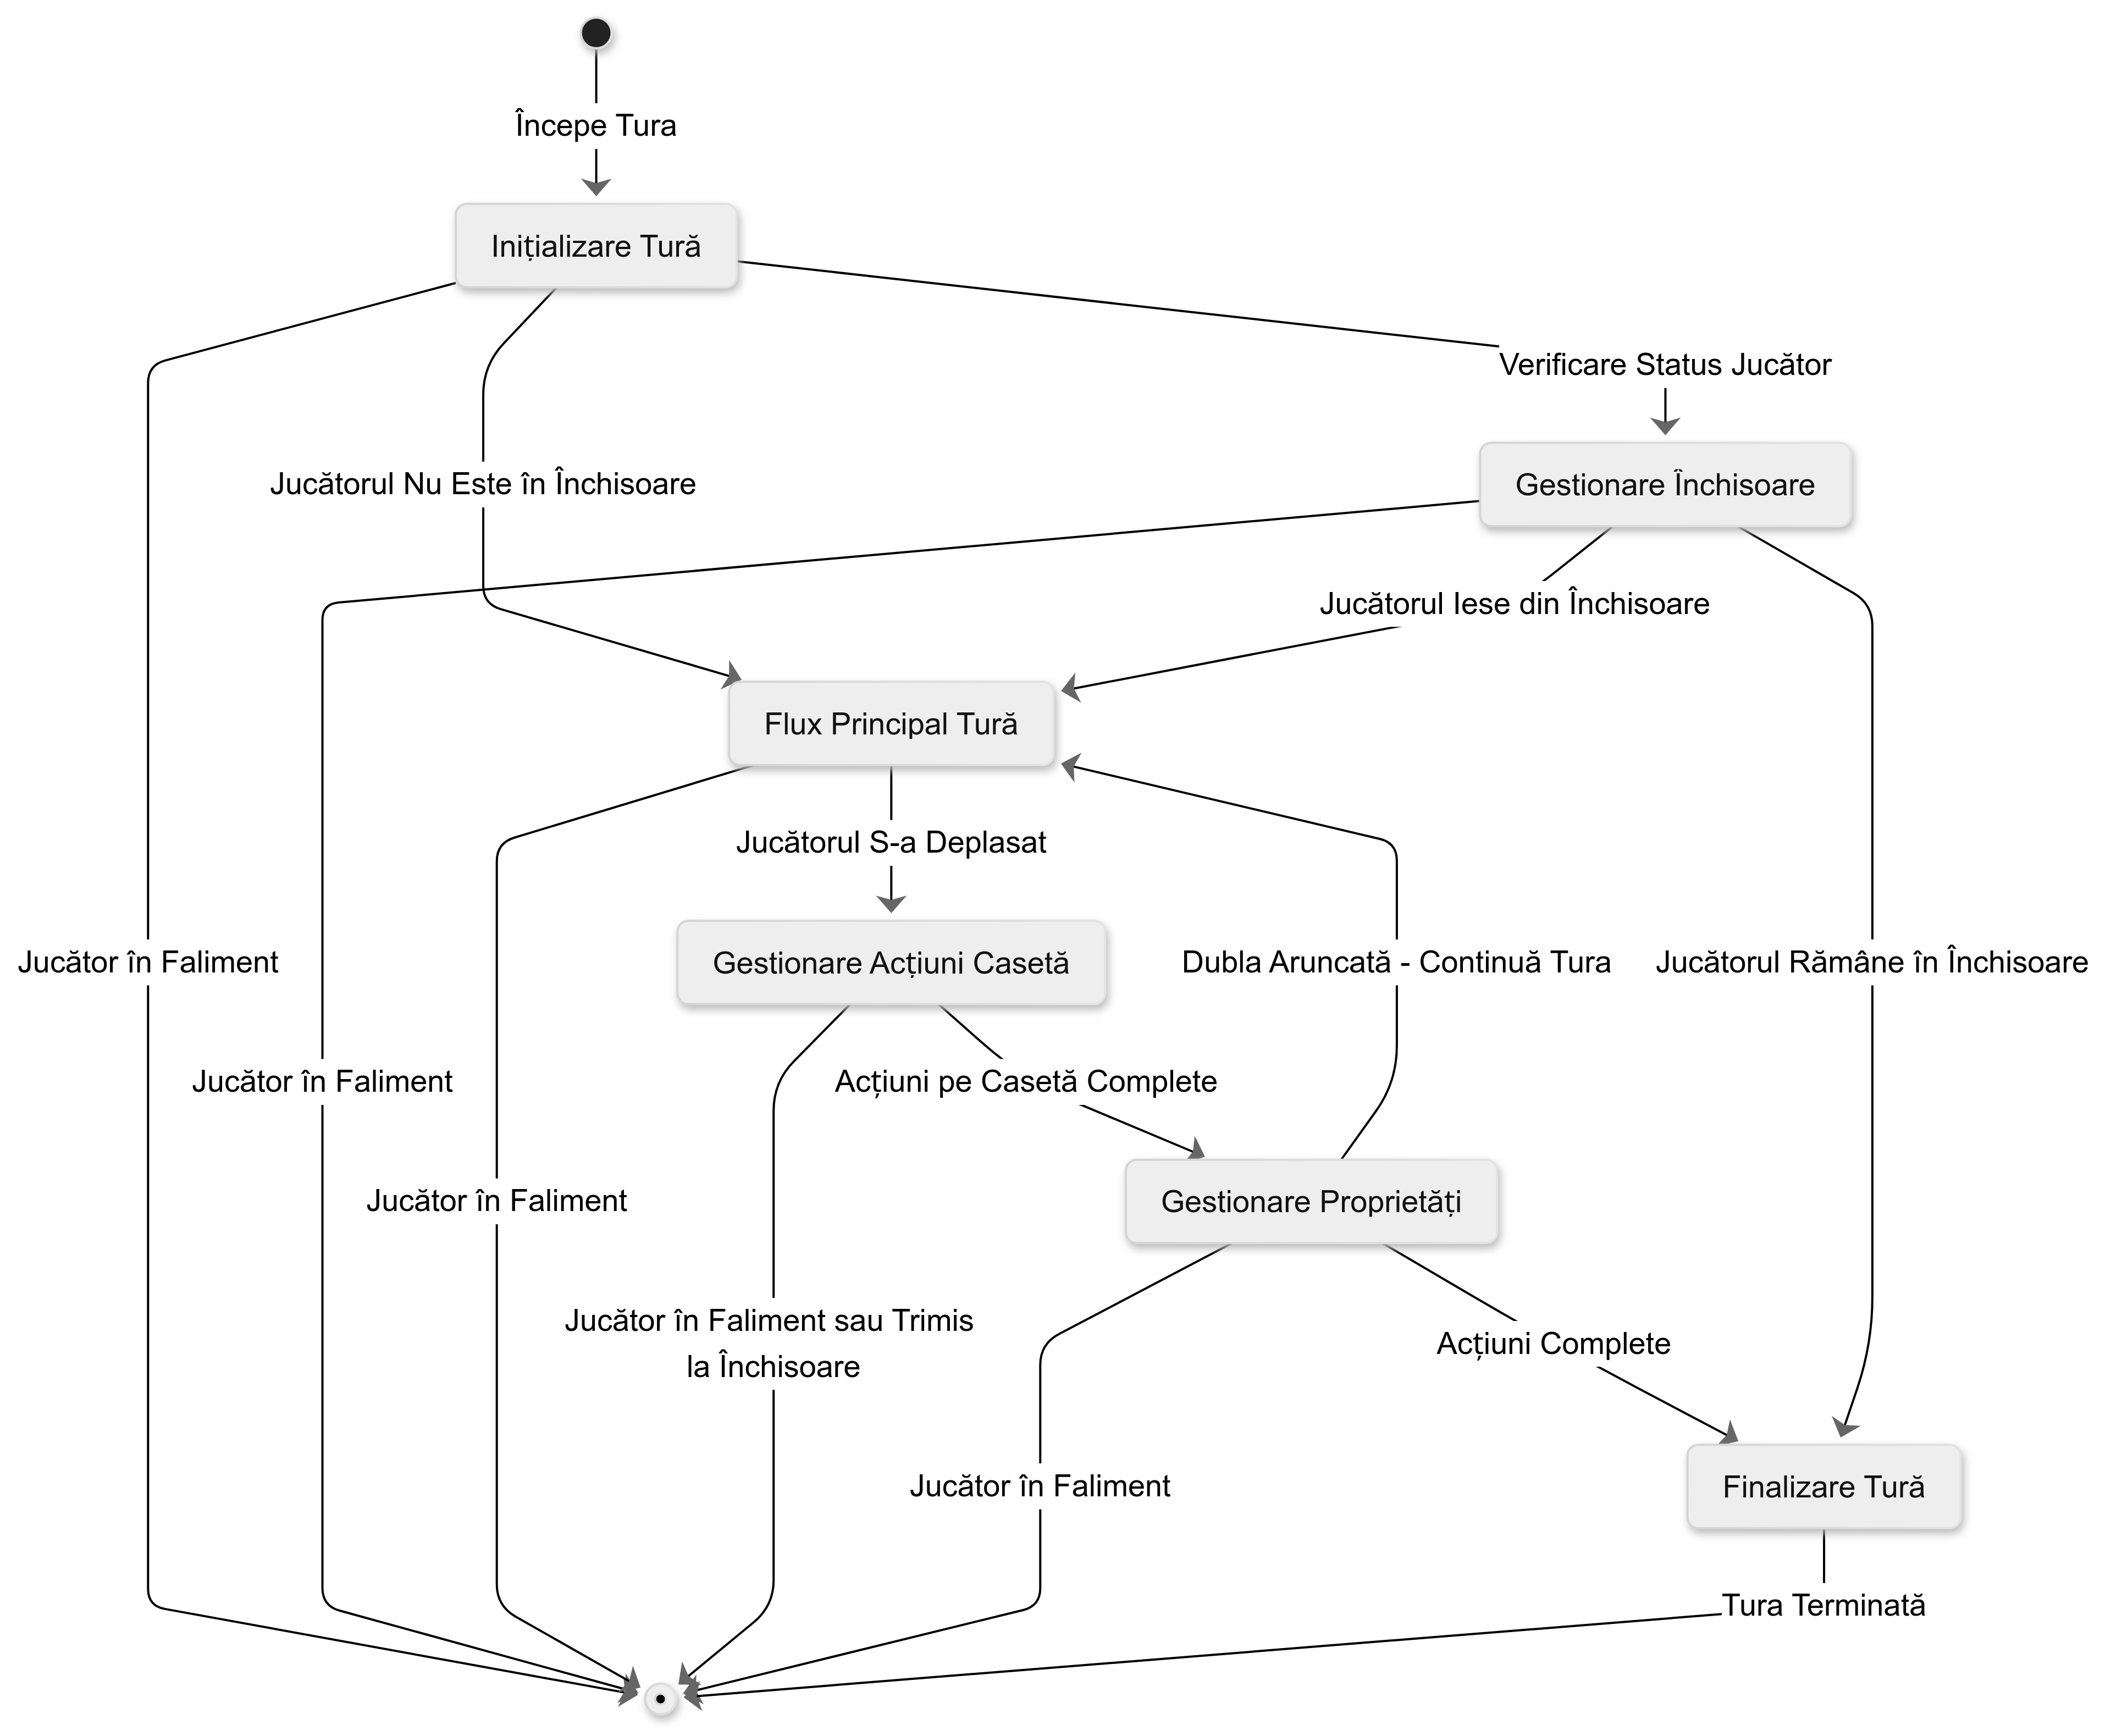
\includegraphics[width=16cm]{images/turn_state_diagram_overview.png}
    \caption{Diagrama generala a unei ture de Monopoly}
    \label{fig:turn_state_diagram_overviewl}
\end{figure}

\begin{figure}[p]
    \centering
    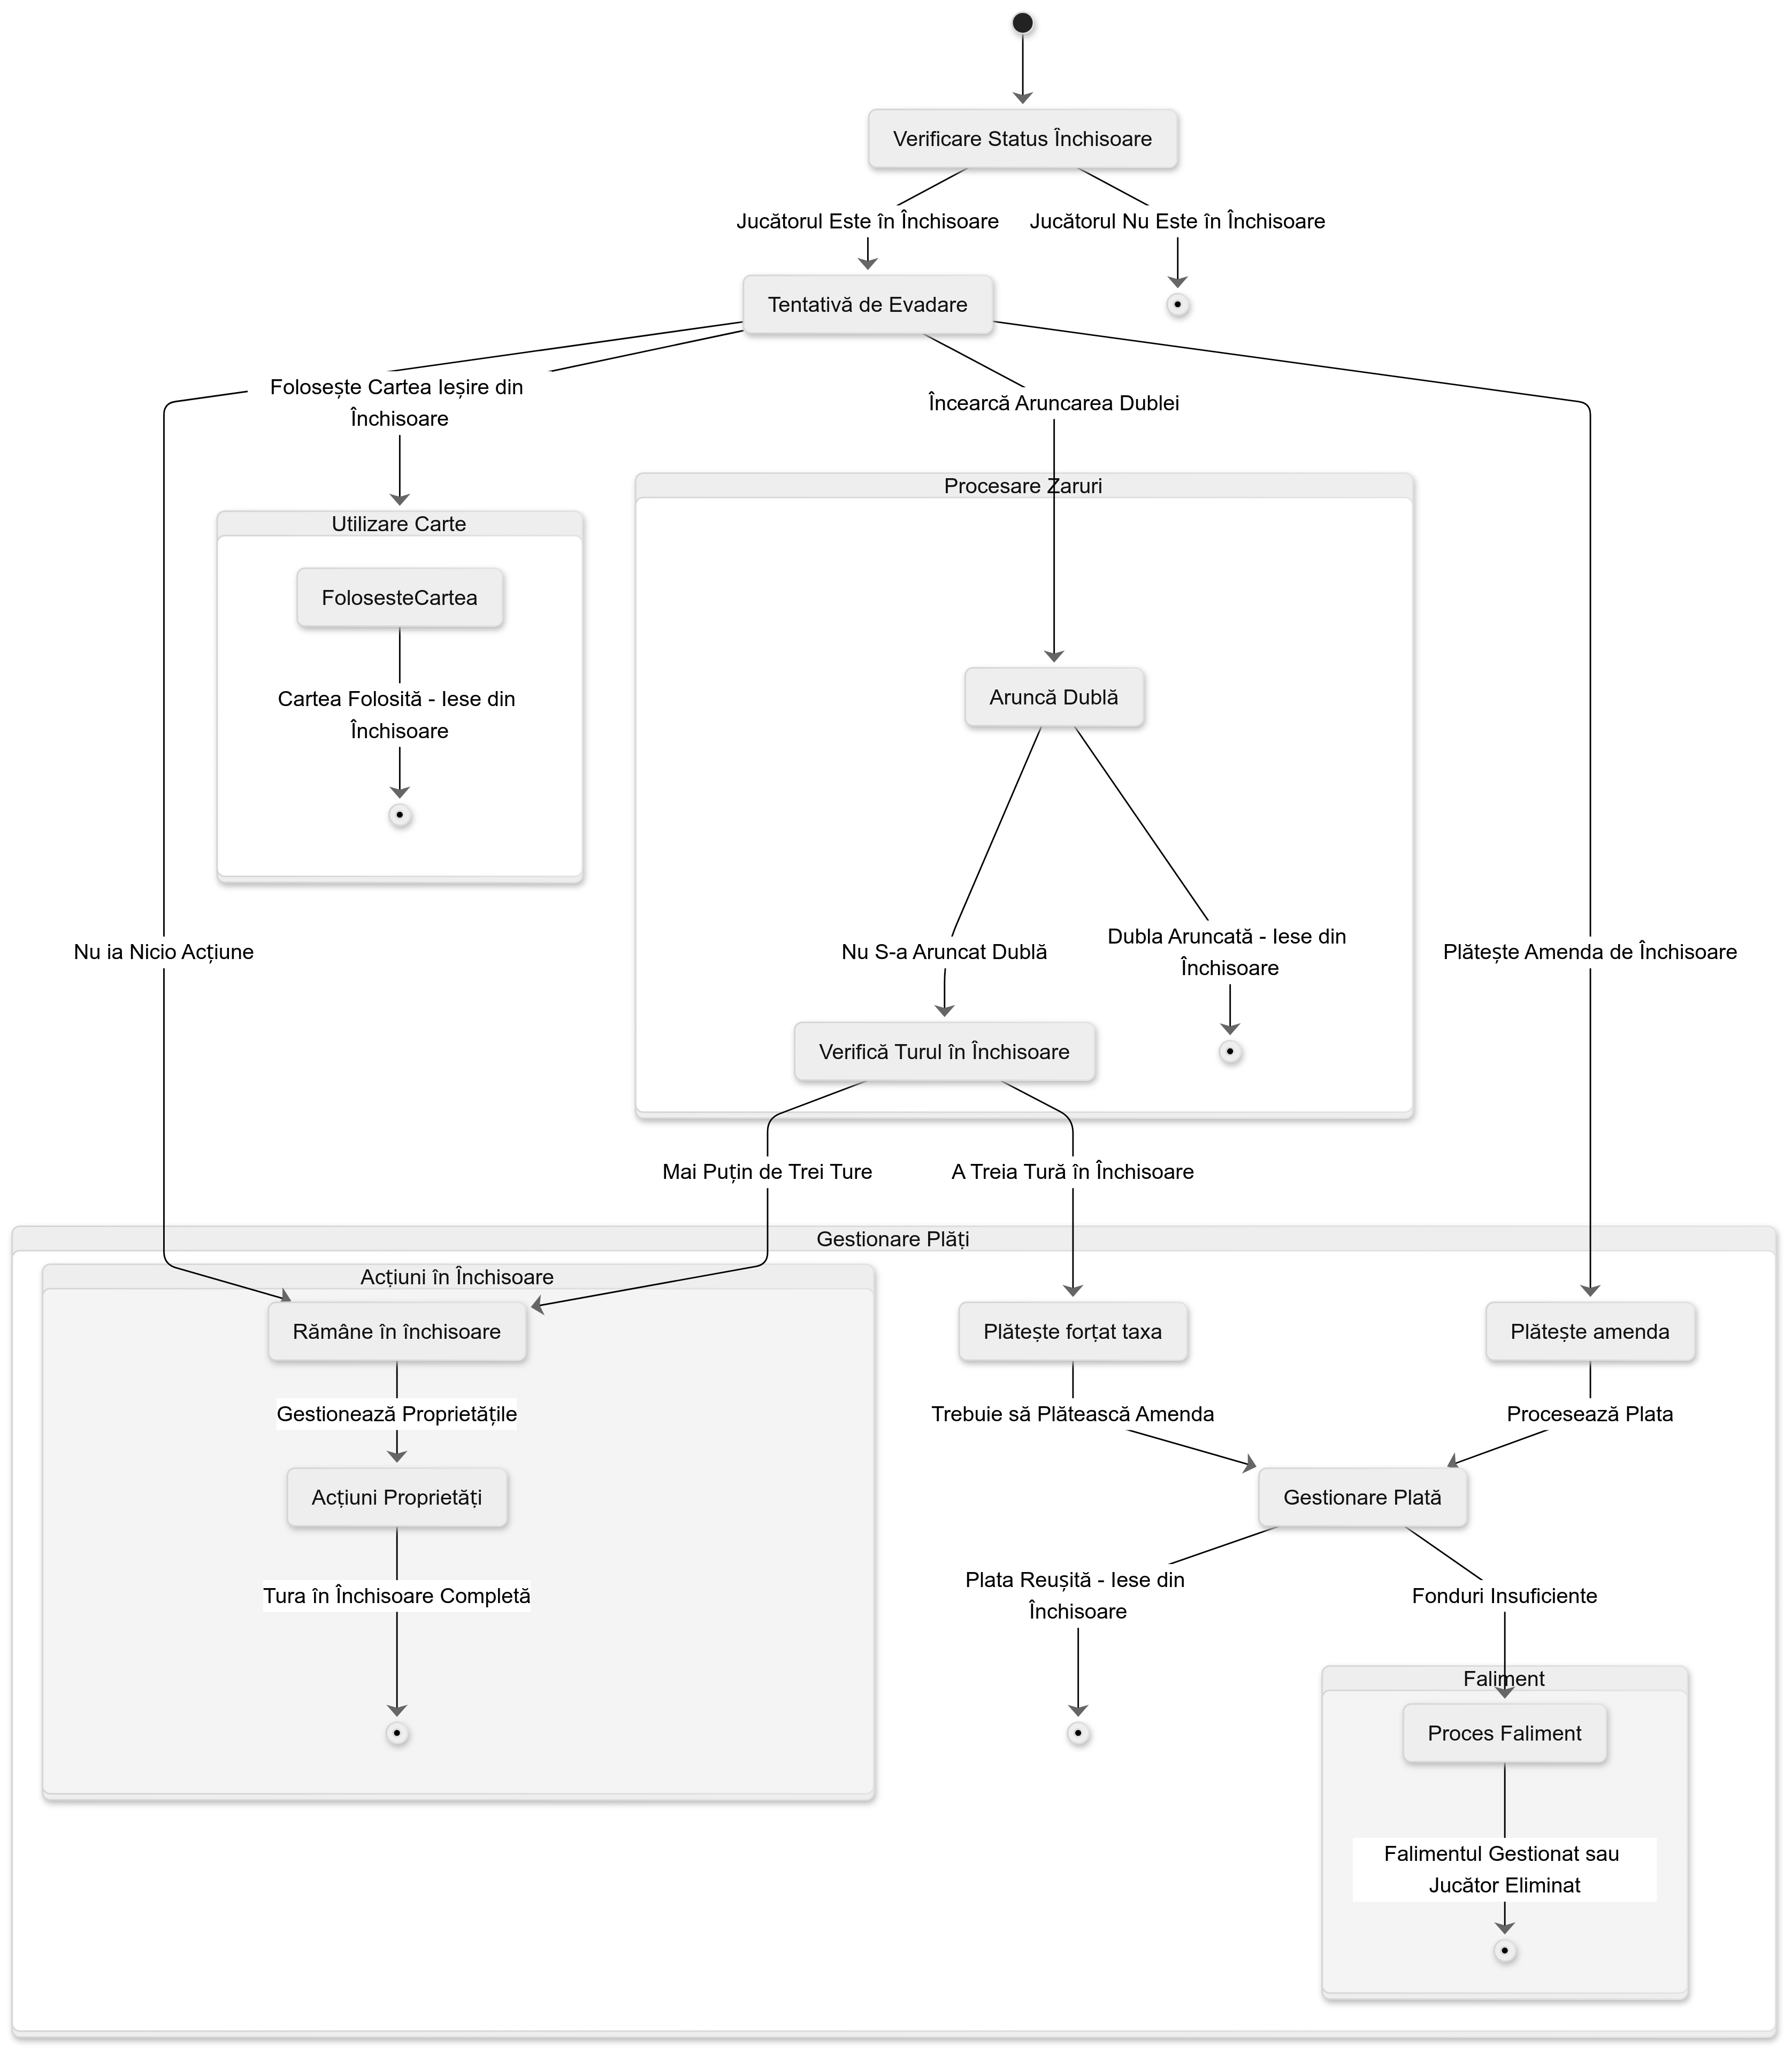
\includegraphics[width=14cm]{images/turn_state_diagram_jail_handler.png}
    \caption{Diagrama de stare a acțiunilor întreprinse în închisoare}
    \label{fig:turn_state_diagram_overviewl}

    % helps with vertical centering
    \begin{minipage}{.1cm}
        \vfill
    \end{minipage}
\end{figure}

\begin{figure}[H]
    \centering
    \rotatebox{270}{%
        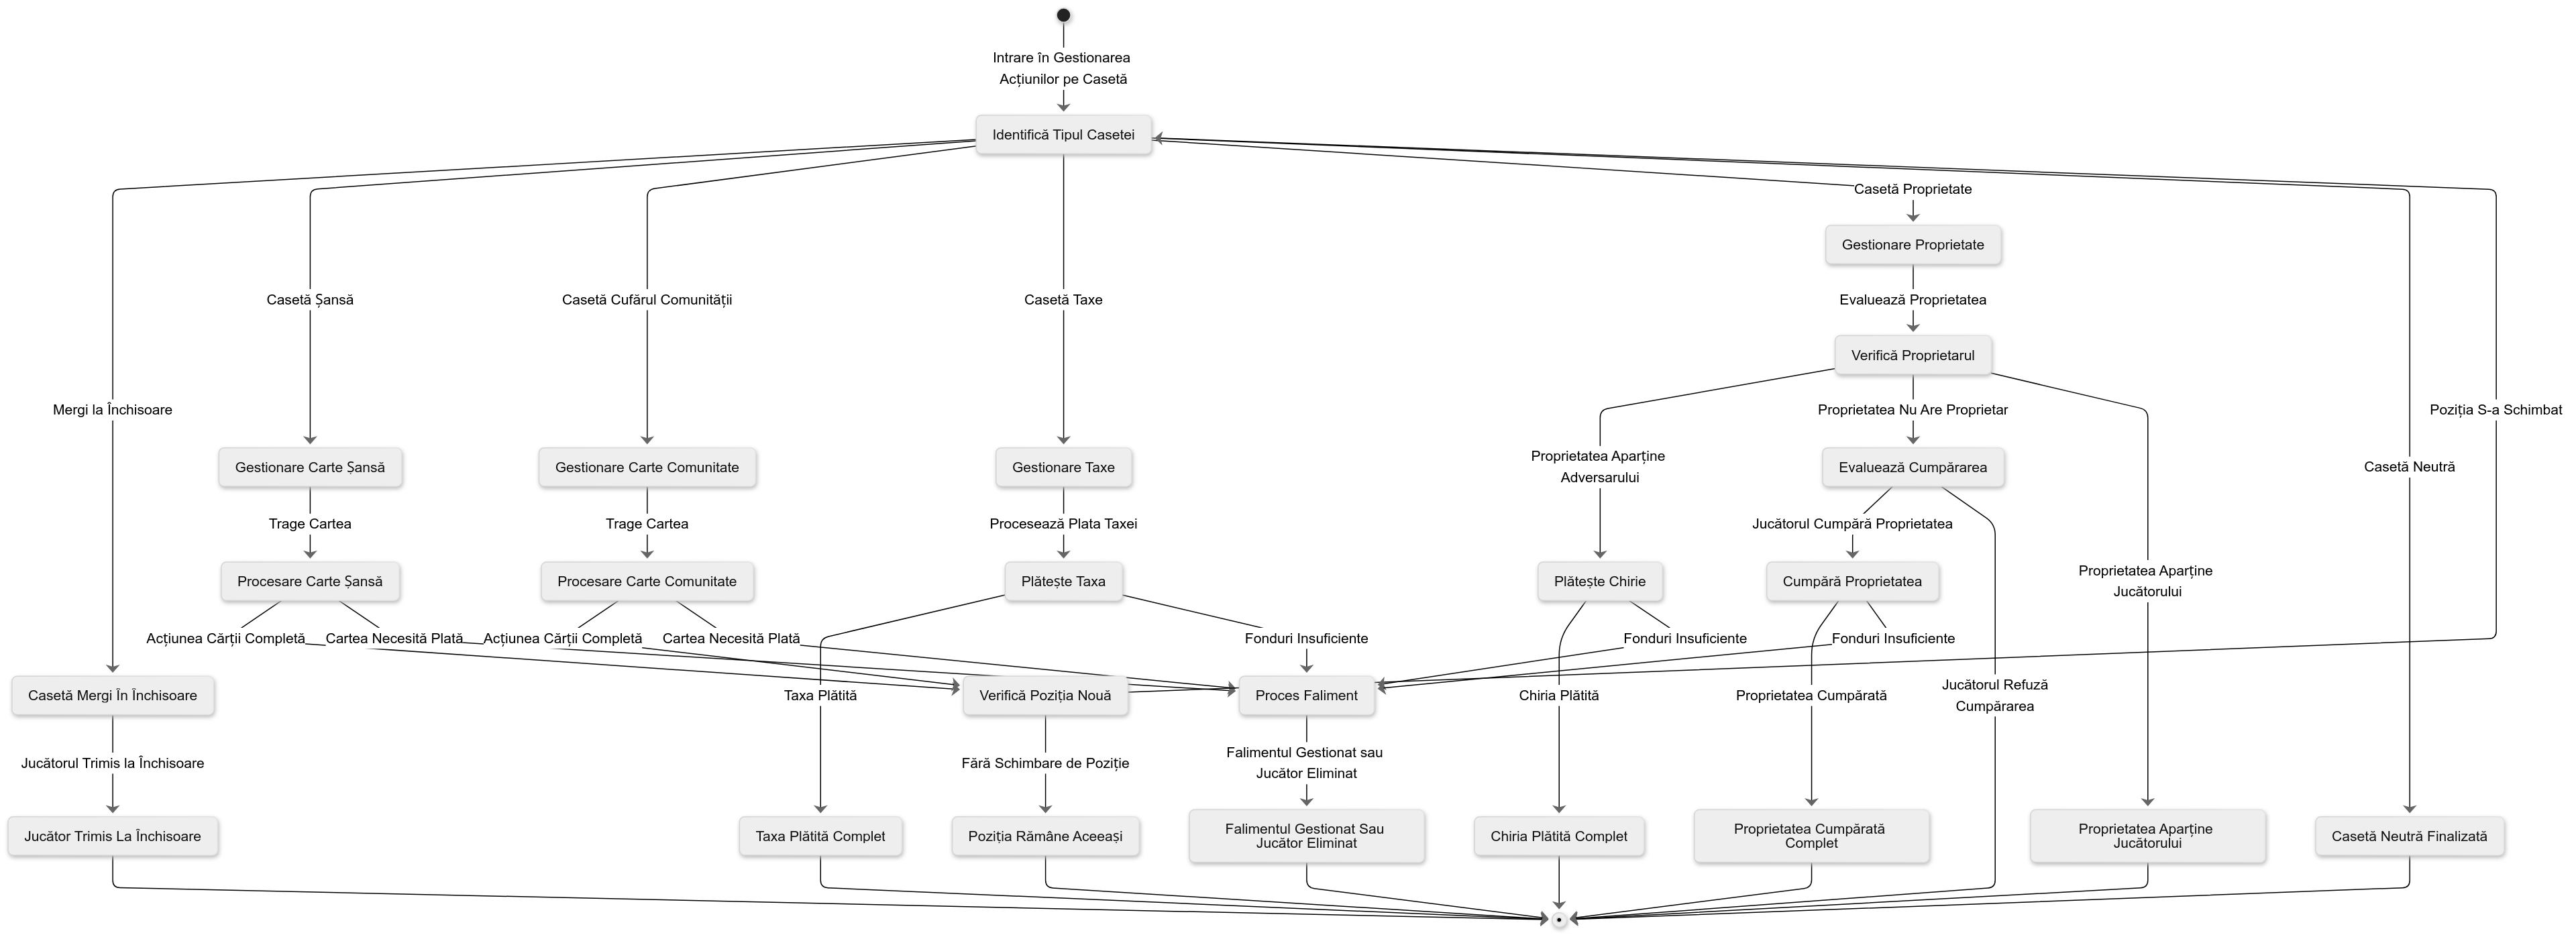
\includegraphics[width=24cm]{images/turn_state_diagram_tile_handler.png}
    }
    \caption{Diagrama de stare a acțiunilor întreprinse după o aruncare de zaruri}
    \label{fig:turn_state_diagram_overviewl}
\end{figure}

\begin{figure}[H]
    \centering
    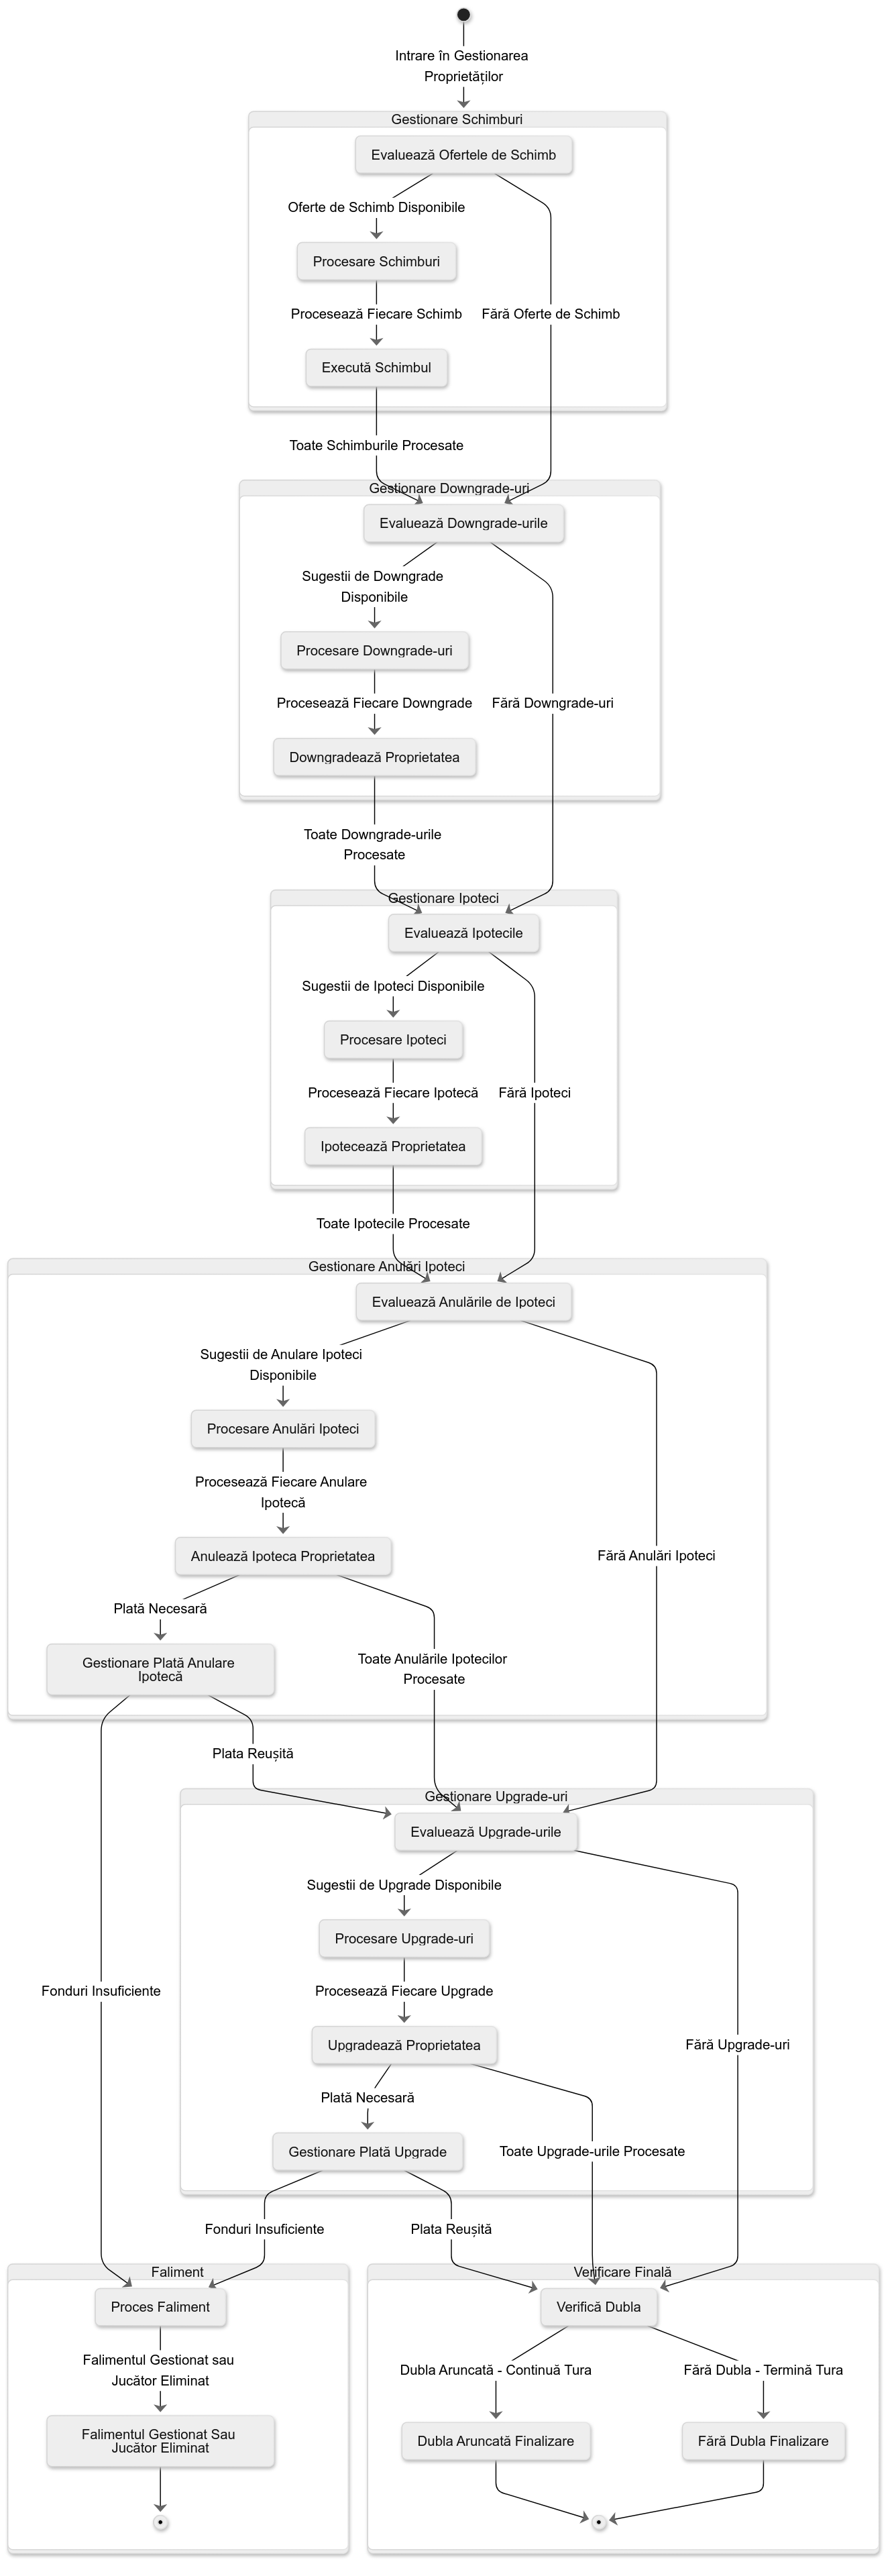
\includegraphics[height=24cm]{images/turn_state_diagram_property_actions.png}
    \caption{Diagrama de stare a acțiunilor pentru proprietăți}
    \label{fig:turn_state_diagram_overviewl}
\end{figure}
\end{appendix}

\printbibliography[heading=bibintoc]

\end{document}